\RequirePackage[T1]{fontenc}
\documentclass[conference,letterpaper,10pt,onecolumn]{IEEEtran}
\usepackage[T1]{fontenc}
\usepackage{mathptmx}
\usepackage{amsmath,amssymb}
\usepackage{graphicx}
\usepackage{booktabs,array,tabularx}
\usepackage{float}
\usepackage{xcolor}
\usepackage{url}
\usepackage[hidelinks]{hyperref}
\usepackage{cite}
\graphicspath{{figures/}}
\newcommand{\E}{\mathbb{E}}
\newcommand{\ind}{\mathbf{1}}
\newcommand{\conpath}{ConPath}
\newcommand{\valonly}{\textbf{Development validation only.}}
\newcommand{\workingnote}{\begin{center}\small\textbf{Anonymous working draft --- 10 September 2026}\\Validation-only evidence; not a submission-ready or final-test report.\end{center}}
\setlength{\emergencystretch}{1em}
\renewcommand{\arraystretch}{1.12}
\renewcommand{\topfraction}{0.85}
\renewcommand{\dbltopfraction}{0.85}
\renewcommand{\textfraction}{0.1}
\pagestyle{plain}

\title{ConPath: Joint Spatial Map Posteriors for\\Footprint-Aware Reachability Prediction\\\large Supplementary Evidence and Reproducibility Record}
\author{\IEEEauthorblockN{Anonymous working draft}}
\renewcommand{\thepage}{S-\arabic{page}}
\begin{document}
\maketitle
\workingnote
\begin{abstract}
This supplement preserves the full existing-evidence comparison, protocol differences, missing measurements, counterexamples, and fixed qualitative cases behind the main working manuscript. It is a record of development validation and historical diagnostics, not a final-test report. No additional model training, model inference, calibration fitting, query revision, or final-test reading is required to typeset these files. All numerical tables are converted from the project's existing auditable summaries. The LaMa BEV adaptation and FM+XAttn literature reimplementation remain under-converged supplementary engineering records; external training is stopped.
\end{abstract}

\section{Evidence Cohorts and Claims}
\textbf{D1: current parent-isolated development.} Five indoor sources contribute 20/5/8 parent places apiece, for 100 training, 25 selection, and 40 validation places, with one observation per place. Validation has 515 terminal queries and 1,545 events at radii 0/10/20 cells. ConPath, independent, and deterministic models have three seeds: 20260910, 20260911, 20260912. All current packets derive from the physical training archive; recorded parent overlap and cross-split exact D4 duplicates are zero. Data preparation inspected development references and validation was later reused to choose a sampling modification. These are bounded development experiments, not unseen final-test confirmation.

\textbf{D2: existing two-seed sampling exploration.} The correlated categorical-noise candidate uses the same 100/25/40 cohort but only seeds 20260910/20260911. Comparisons use those same two seeds in every row. It uses a $9\times9$, $\sigma=3$ Gaussian-copula categorical-noise field, with unchanged learned parameter count but additional computation. It is not the paper's selected method and is not pooled with D1's three-seed means.

\textbf{H1: historical diagnostic.} The six-method comparison has 160 training and 160 validation observations; 142 validation subscenes contribute 1,408 terminal groups and 4,224 events. Stochastic evaluation uses $K=128$. The full/independent/no-event/no-global and deterministic families use seeds 20260831/20260901/20260902, while direct-query has only seed 20260831. Later audits found that 27 of the 160 validation \emph{observations} share a parent place with training. The 142 subscenes are not established independent parent places. This cohort supports conditional mechanism diagnostics, not unseen-place generalization. The fixed-marginal intervention and mean-map controls use this same cohort and remain separate from D1.

\textbf{S1 and stopped external records.} P0 synthetic held-out-template reports are separate from FlatLands; the full model has two seeds and the matched no-event comparison one. They are not inserted into D1 or H1 tables. The independently frozen external protocol has 985/97/191 training/calibration/validation places, with no matched ConPath result used here. LaMa/FM staging was cancelled, and these observations do not fill D1's missing rows.

\textbf{Interpretation of uncertainty.} Reported $\pm$ values are sample SD across training seeds. Existing paired bootstrap intervals condition on the recorded seed means and retain their original parent or subscene resampling unit. Generated worlds, query rows, and multiple views of the same place are not extra independent training repeats. Historical overlap cannot be repaired by a subscene bootstrap.

\section{Protocol, Model, and Selection Freeze}
The input remains free/blocked/unknown BEV channels with separately supplied valid support. Hidden-map scores use valid unobserved cells. Every within-cohort method shares the input, labels, queries, masks, footprint radii, weighting, and exact evaluation contract. In D1, query generation is input-defined and retains goals blocked in the reference. Radius is in grid cells; no meter conversion is asserted.

The original ConPath uses a width-16 U-Net with pooled global context and coordinates; its decoder has four low-rank Gaussian factors and a $5\times5$ variance-normalized local Gaussian logit field. Independent disables global factors and changes the local kernel to one cell, retaining map and event training losses. No-global removes low-rank decoder factors only, not encoder context or local correlation. No-event sets event-loss weight to zero but still uses the common event-based checkpoint-selection rule. The separately trained deterministic model does not have ConPath's four-dimensional latent decoder. Direct-query is not relabeled as the distinct coordinate-query control.

Known and support-invalid cells have $+10/-10$ class logits before registered unit-scale independent Gumbel sampling. Uniform draws are clipped to $[10^{-6},1-10^{-6}]$; the fixed logit gap protects hard-world constraints at that scale. Continuous marginals are separately projected by the evaluator. The original implementation does not contain an arbitrary-scale hard projection after sampling. The ideal conditional softmax identity has a numerical clipping approximation. These implementation details limit claims about the model class beyond the registered sampler.

Current optimization uses AdamW with learning rate $3\times10^{-4}$, weight decay $10^{-4}$, gradient norm clipping 5, effective batch 4/micro-batch 2; training $K=4$, selection $K=16$. The budget is at most 24 epochs/600 updates with the archived early-stopping rule. The selection checkpoint minimizes Event Brier on 25 separate places, breaking ties within $10^{-5}$ using map NLL. The hard forward event is corrected to exact connectivity; the backward path retains a bounded 256-step relaxed surrogate. Two zero-query training places expose a shared micro-batch event-weighting limitation. The historical training/selection forward operator was bounded, with separate exact final evaluation; that protocol is not identical to the current one.

\begin{table}[H]
\centering\small
\caption{Selected original ConPath checkpoints. No best-seed selection or ensemble is used; all three original selection checkpoints are retained. Paths are relative to the project root.}
\begin{tabular}{@{}lccp{4.1in}@{}}\toprule
Seed & Selected epoch & Trained epochs & Checkpoint under \texttt{results/parent\_group\_pilot\_v1/runs/}\\\midrule
20260910 & 21 & 24 & \texttt{correlated/20260910/best.pt}\\
20260911 & 17 & 23 & \texttt{correlated/20260911/best.pt}\\
20260912 & 22 & 24 & \texttt{correlated/20260912/best.pt}\\\bottomrule
\end{tabular}
\end{table}
The corresponding checkpoint SHA-256 values are, in seed order:
\begin{quote}\footnotesize\ttfamily
\nolinkurl{a1cc966191aa5d5526738dce648a3d42c57aedddf3218b979f3f5266fc69bc73}\\
\nolinkurl{d4dc1e0becf492e037c723548c9c7e3a3098cd7c894552a02fd0f1cb64740618}\\
\nolinkurl{284584c5dfbaac6a335759d6eb46a6480aae77508443171b4ff2e640e4456ab0}
\end{quote}
Existing ConPath Brier is lower than independent in all three current seeds, satisfying the requested stopping condition. No new A/B/C optimization, temperature fit, third candidate seed, external model training, or threshold change is started. Selection and checkpoint identities remain fixed.

\section{Current Development Tables}
\begin{table}[H]\centering\small
\caption{D1 compact six-method matrix (source table T1). Three seeds, equal-parent weighting. Hidden-map Brier here is the hard-world free-frequency score; deterministic $K=1$ is binary-map squared error, not its continuous probability score. Risk30 means risk at equal 30\% coverage. Missing measurements are not zero.}
% Generated from immutable reported values; no model inference.
\resizebox{\linewidth}{!}{\begin{tabular}{@{}lrrrrr@{}}\toprule
Method & Actual K & Seeds & Event Brier $\downarrow$ & Risk at 30\% coverage $\downarrow$ & Hidden-map Brier $\downarrow$\\\midrule
Deterministic occupancy & 1 & 3 & 0.11152 $\pm$ 0.00256 & 0.25164 $\pm$ 0.01024 & 0.18988\\
Independent Bernoulli & 32 & 3 & 0.11201 $\pm$ 0.00366 & 0.24432 $\pm$ 0.00928 & 0.15402\\
Direct-query & --- & 0 & Not evaluated & --- & ---\\
No-global & --- & 0 & Not evaluated & --- & ---\\
No-event & --- & 0 & Not evaluated & --- & ---\\
ConPath & 32 & 3 & 0.10380 $\pm$ 0.00350 & 0.23952 $\pm$ 0.00578 & 0.15388\\
\bottomrule\end{tabular}}

\end{table}
The recorded interval for the Brier difference (independent minus ConPath) is $[0.00439,0.01251]$. For deterministic minus ConPath it is $[-0.01616,0.03377]$. These existing intervals use source-stratified paired-parent resampling conditional on the three seed means. Only the former excludes zero, within this development cohort.

\begin{table}[H]\centering\small
\caption{D1 retrospective metrics (T1b), from unchanged saved predictions. NLL clips at $10^{-6}$; ECE uses ten equal-width bins. These additional summaries were not original model-selection criteria. Continuous hidden-map Brier uses deterministic sigmoid probabilities and the stochastic $K=32$ conditional-probability average.}
% Generated from immutable reported values; no model inference.
\resizebox{\linewidth}{!}{\begin{tabular}{@{}lrrrrrr@{}}\toprule
Method & Actual K & Event NLL $\downarrow$ & Event ECE $\downarrow$ & False-safe @0.8 $\downarrow$ & Coverage @0.8 & Continuous hidden-map Brier $\downarrow$\\\midrule
Deterministic occupancy & 1 & 1.54065 $\pm$ 0.03537 & 0.11152 $\pm$ 0.00256 & 0.25164 $\pm$ 0.01024 & 0.34198 $\pm$ 0.00883 & 0.13869 $\pm$ 0.00542\\
Independent Bernoulli & 32 & 0.94364 $\pm$ 0.06507 & 0.10131 $\pm$ 0.00578 & 0.20847 $\pm$ 0.01295 & 0.22453 $\pm$ 0.01525 & 0.15158 $\pm$ 0.00852\\
ConPath & 32 & 0.79330 $\pm$ 0.10289 & 0.08622 $\pm$ 0.00315 & 0.18649 $\pm$ 0.01396 & 0.21340 $\pm$ 0.00842 & 0.15147 $\pm$ 0.00378\\
\bottomrule\end{tabular}}

\end{table}
Deterministic completion's continuous Brier is better than ConPath's. Its thresholded binary score must not be substituted to manufacture a probabilistic mapping advantage. NLL and ECE alone are also insufficient: a train-fitted radius prior below has better values than ConPath but no threshold-0.8 acceptance.

\begin{table}[H]\centering\small
\caption{D1 saved $K=4$ prefix versus $K=32$ (T1c). Same checkpoints and queries; no new inference. Zero score-monotonicity violations are structural checks and are not calibration guarantees.}
% Generated from immutable reported values; no model inference.
\resizebox{\linewidth}{!}{\begin{tabular}{@{}lrrrrrr@{}}\toprule
Method & K & Brier $\downarrow$ & ECE $\downarrow$ & False-safe @0.8 $\downarrow$ & Coverage @0.8 & Radius monotonicity violations\\\midrule
ConPath & 4 & 0.11064 $\pm$ 0.00666 & 0.09633 $\pm$ 0.00698 & 0.17801 $\pm$ 0.01356 & 0.19624 $\pm$ 0.00358 & 0\\
ConPath & 32 & 0.10380 $\pm$ 0.00350 & 0.08622 $\pm$ 0.00315 & 0.18649 $\pm$ 0.01396 & 0.21340 $\pm$ 0.00842 & 0\\
Independent Bernoulli & 4 & 0.12028 $\pm$ 0.00844 & 0.10985 $\pm$ 0.01085 & 0.20673 $\pm$ 0.01934 & 0.21058 $\pm$ 0.01425 & 0\\
Independent Bernoulli & 32 & 0.11201 $\pm$ 0.00366 & 0.10131 $\pm$ 0.00578 & 0.20847 $\pm$ 0.01295 & 0.22453 $\pm$ 0.01525 & 0\\
\bottomrule\end{tabular}}

\end{table}
All 23 current method/seed/budget files retain 515 radius triples with zero score/target radius-monotonicity violations. Existing saved-world audits report zero observed-evidence and valid-support violations. No fresh geometry audit is implied by this typesetting step. Per-query calibration predictions were not archived; unavailable calibration NLL/ECE cannot be reconstructed honestly from aggregate selection scores.

\begin{table}[H]\centering\small
\caption{D1 fixed rule controls (T1d). Rules have one deterministic evaluation, not three optimization seeds. The radius prior has no sampled map; its archived $K=1$ filename tag is not a map count. A dash at zero coverage means undefined risk.}
% Generated from immutable reported values; no model inference.
\resizebox{\linewidth}{!}{\begin{tabular}{@{}lrrrrrr@{}}\toprule
Control & Actual maps & Brier $\downarrow$ & NLL $\downarrow$ & ECE $\downarrow$ & False-safe @0.8 $\downarrow$ & Coverage @0.8\\\midrule
All unknown free & 1 & 0.18048 & 2.49341 & 0.18048 & 0.39087 & 0.46174\\
All unknown blocked & 1 & 0.28126 & 3.88578 & 0.28126 & --- & 0.00000\\
Nearest observed & 1 & 0.13834 & 1.91117 & 0.13834 & 0.30460 & 0.36573\\
Train-fitted radius prior & N/A & 0.15606 & 0.48499 & 0.05653 & --- & 0.00000\\
\bottomrule\end{tabular}}

\end{table}

\begin{table}[H]\centering\small
\caption{D1 previously saved post-hoc conditional-mean threshold controls (T1e). The threshold remains 0.5 and each output is one binary map. These are distinct from the separately trained deterministic baseline. NLL/ECE were not stored and are not fabricated.}
% Generated from immutable reported values; no model inference.
\resizebox{\linewidth}{!}{\begin{tabular}{@{}lrrr@{}}\toprule
Derived output & Actual maps & Event Brier $\downarrow$ & Risk at 30\% coverage $\downarrow$\\\midrule
ConPath same-checkpoint conditional-mean threshold & 1 & 0.11410 $\pm$ 0.00301 & 0.27791 $\pm$ 0.00724\\
Independent same-checkpoint conditional-mean threshold & 1 & 0.11640 $\pm$ 0.00694 & 0.27739 $\pm$ 0.01524\\
\bottomrule\end{tabular}}

\end{table}
The known-immutable subset contains 750/1,545 events (unweighted) with zero ConPath error. On the hidden-completion-mutable subset, ConPath's parent-weighted Brier is $0.19912\pm0.00967$. Full-cohort and subset metrics each use their own contributing-parent normalization. The saved diagnostic predates manuscript consolidation; it is not a new evaluation.

\begin{table}[H]\centering\small
\caption{D1 descriptive radius strata from the unchanged numeric snapshot. Three seeds; equal-parent normalization within each radius. Brier is mean $\pm$ sample SD; other displayed values are seed means. Undefined threshold risk is retained when no seed accepts any event. Radii are grid cells.}
% Generated from immutable reported values; no model inference.
\resizebox{\linewidth}{!}{\begin{tabular}{@{}lrrrrrr@{}}\toprule
Method & K & Radius (cells) & Event Brier $\downarrow$ & ECE $\downarrow$ & False-safe @0.8 & Coverage @0.8\\\midrule
ConPath & 32 & 0 & 0.15329 $\pm$ 0.01047 & 0.12824 & 0.17754 & 0.60473\\
ConPath & 32 & 10 & 0.09668 $\pm$ 0.00783 & 0.07830 & 0.30851 & 0.03547\\
ConPath & 32 & 20 & 0.06142 $\pm$ 0.00804 & 0.06179 & Undefined & 0.00000\\
Deterministic & 1 & 0 & 0.18790 $\pm$ 0.00759 & 0.18790 & 0.19302 & 0.66478\\
Deterministic & 1 & 10 & 0.10639 $\pm$ 0.00662 & 0.10639 & 0.39336 & 0.24830\\
Deterministic & 1 & 20 & 0.04025 $\pm$ 0.00425 & 0.04025 & 0.28529 & 0.11286\\
Independent & 32 & 0 & 0.16474 $\pm$ 0.01352 & 0.14892 & 0.18898 & 0.59613\\
Independent & 32 & 10 & 0.10249 $\pm$ 0.01566 & 0.09479 & 0.34346 & 0.07316\\
Independent & 32 & 20 & 0.06880 $\pm$ 0.00752 & 0.06997 & 0.41239 & 0.00430\\
\bottomrule\end{tabular}}

\end{table}
At radius 20 ConPath has zero threshold-0.8 coverage in every seed, and deterministic completion has lower Brier. Radius-10 ConPath coverage is also low. These strata prevent interpreting an overall Brier improvement or score monotonicity as reliable high-confidence reachability for every robot footprint. Source, reachable/unreachable, pooled, and parent-weighted metrics remain in the machine-readable snapshot and companion CSV exports.

\clearpage
\section{Historical Mechanism and Ablation Diagnostics}
\textbf{This section is H1, not D1.} The later audit found training-parent overlap in 27/160 validation observations and historical physical archive-test access. The $K=128$ and subscene-weighted results below cannot fill D1's missing $K=32$ rows or support untouched-place conclusions.

\begin{table}[H]\centering\small
\caption{H1 historical six-method table (T2). Three training seeds 20260831/0901/0902 except direct-query (20260831 only). Common within-table evaluation does not repair parent overlap. Seed counts are shortened for typesetting; source tables preserve exact identifiers.}
% Generated from immutable reported values; no model inference.
\resizebox{\linewidth}{!}{\begin{tabular}{@{}lrrrrrrr@{}}\toprule
Method & Actual K & Seed count & Event Brier $\downarrow$ & Event NLL $\downarrow$ & Event ECE $\downarrow$ & False-safe @0.8 $\downarrow$ & Coverage @0.8\\\midrule
Deterministic occupancy & 1 & 3 & 0.08857 $\pm$ 0.00323 & 1.22362 $\pm$ 0.04463 & 0.08857 $\pm$ 0.00323 & 0.07293 $\pm$ 0.00682 & 0.44278 $\pm$ 0.01024\\
Independent Bernoulli & 128 & 3 & 0.09521 $\pm$ 0.00703 & 0.78503 $\pm$ 0.04690 & 0.08720 $\pm$ 0.00741 & 0.05689 $\pm$ 0.00832 & 0.36592 $\pm$ 0.01692\\
Direct-query & N/A & 1 & 0.09119 & 0.29788 & 0.04076 & 0.08335 & 0.37412\\
No-global & 128 & 3 & 0.09499 $\pm$ 0.00157 & 0.78486 $\pm$ 0.05495 & 0.08592 $\pm$ 0.00058 & 0.05739 $\pm$ 0.01662 & 0.36354 $\pm$ 0.00957\\
No-event & 128 & 3 & 0.20425 $\pm$ 0.00322 & 2.53067 $\pm$ 0.05699 & 0.21690 $\pm$ 0.01933 & 0.02561 $\pm$ 0.01609 & 0.19316 $\pm$ 0.10435\\
ConPath & 128 & 3 & 0.06749 $\pm$ 0.00936 & 0.28854 $\pm$ 0.01662 & 0.05715 $\pm$ 0.00683 & 0.04552 $\pm$ 0.01429 & 0.33644 $\pm$ 0.00579\\
\bottomrule\end{tabular}}

\end{table}
Full/no-event/no-global within-seed Brier intervals favor full, but their subscene resampling unit is not independent buildings. The direct-query row has lower ECE than ConPath's three-seed mean and only one seed. No-event has lower false-safe risk at threshold 0.8 but lower coverage. At equal 30\% coverage, full/independent risks are 0.03600/0.03901; every recorded within-seed paired interval includes zero. No-event/no-global mean risk30 values are 0.05655/0.04288, with paired intervals also including zero; no-global's point contrast reverses in two seeds. These counterexamples are retained.

\begin{table}[H]\centering\small
\caption{H1 fixed empirical marginals and same-checkpoint deterministic controls (T3). The permutation preserves every saved hard-world cell free count exactly. A mean-map control produces one binary map from the archived $K=128$ posterior estimate.}
% Generated from immutable reported values; no model inference.
\resizebox{\linewidth}{!}{\begin{tabular}{@{}lrrrr@{}}\toprule
Control & Event Brier $\downarrow$ & Event NLL $\downarrow$ & Event ECE $\downarrow$ & Risk at 30\% coverage $\downarrow$\\\midrule
ConPath, K128 & 0.06749 $\pm$ 0.00936 & 0.28854 $\pm$ 0.01662 & 0.05715 $\pm$ 0.00683 & 0.03600 $\pm$ 0.00986\\
Cellwise world-index permutation, K128 & 0.16139 $\pm$ 0.00677 & 1.53947 $\pm$ 0.18205 & 0.16433 $\pm$ 0.01252 & 0.03908 $\pm$ 0.01622\\
ConPath same-checkpoint mean map & 0.06957 $\pm$ 0.00380 & 0.96118 $\pm$ 0.05253 & 0.06957 $\pm$ 0.00380 & 0.10509 $\pm$ 0.01468\\
Independent same-checkpoint mean map & 0.07184 $\pm$ 0.00349 & 0.99248 $\pm$ 0.04822 & 0.07184 $\pm$ 0.00349 & 0.11023 $\pm$ 0.01558\\
\bottomrule\end{tabular}}

\end{table}
The permutation changes sample alignment without changing empirical cell marginals, isolating useful finite-ensemble dependence in this cohort. It is not an independently sampled infinite factorized posterior or a causal account of all separately trained architecture differences. Historical ConPath and independent map Brier differ (0.15451 versus 0.16789), so their ordinary comparison alone cannot establish fixed-marginal RQ1. The ConPath mean-map Brier is close to full and the direction reverses in one seed, preventing a broad stochastic-versus-deterministic claim.

\begin{figure}[H]\centering
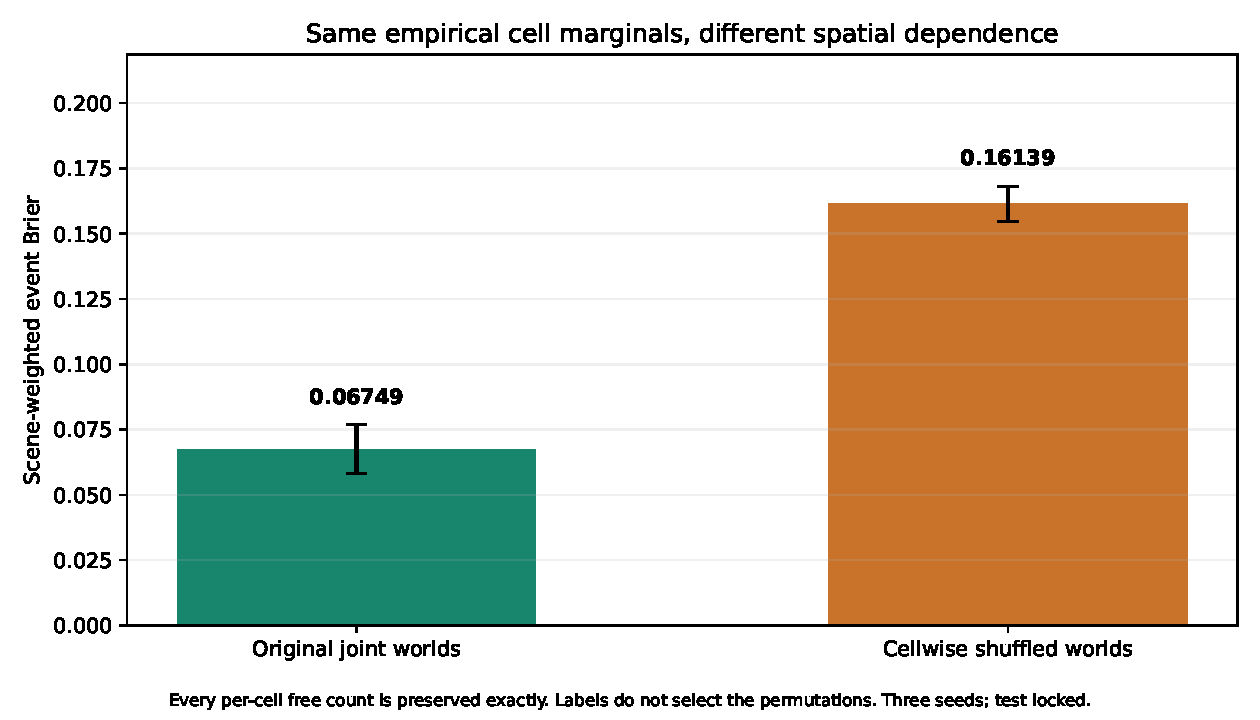
\includegraphics[width=.86\textwidth]{flatlands_clean_marginal_shuffle.pdf}
\caption{Byte-identical archived H1 dependence figure. Despite the old word ``clean'' in the original title/filename, 27/160 historical validation observations share training parent places, and physical archive-test access occurred. This correction overrides earlier untouched/isolated labels. The figure is not evidence of unseen-place generalization.}
\end{figure}

\clearpage
\begin{figure}[H]\centering
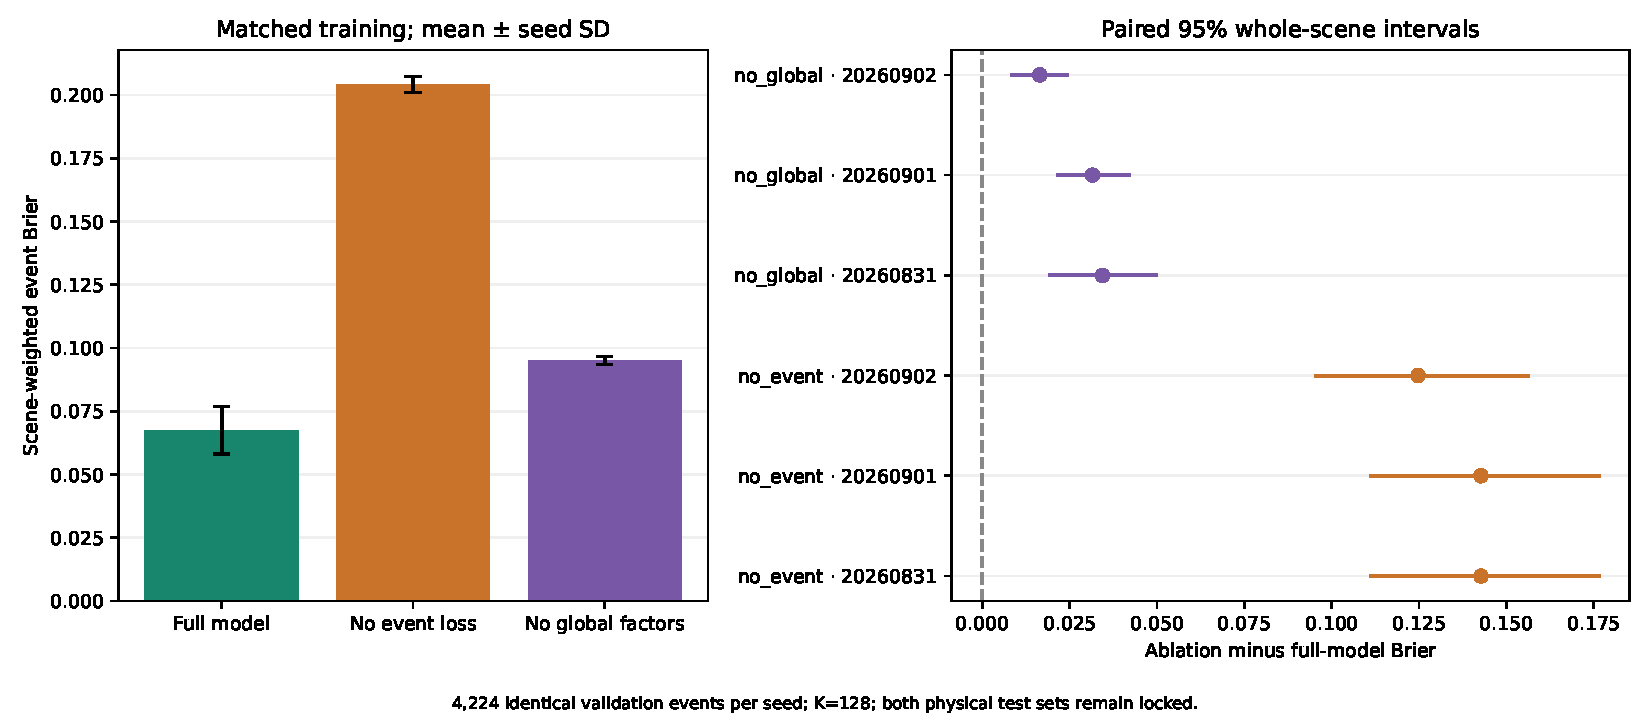
\includegraphics[width=.92\textwidth]{flatlands_clean_training_ablations.pdf}
\caption{Byte-identical H1 historical training ablations, with the same overlap/access caveat. Removing event loss retains event-based selection; removing global decoder factors retains encoder context. Existing intervals are conditional subscene intervals, not independent-building confirmation. Original-language labels are retained; main text and tables provide English method/metric names.}
\end{figure}
The historical no-event model predicts zero reachability for all radius-20 validation queries across three seeds despite a recorded 20.67\% positive rate. This is consistent with fragmented sampled support, not proof that every map-only completion architecture must fail. No corresponding no-event/no-global worlds were saved on D1, so a new parent-isolated qualitative ablation panel is unavailable. Earlier H1 examples selected for positive recovery or avoided false-safe outcomes are excluded from the fixed-case gallery.

\section{Existing Two-seed Sampling Exploration}
\begin{table}[H]\centering\small
\caption{D2 only (T4): the current 100/25/40 cohort restricted to seeds 20260910 and 20260911 for every row. These two-seed means must not be compared directly with D1's three-seed means. The candidate is not selected as the paper method.}
% Generated from immutable reported values; no model inference.
\resizebox{\linewidth}{!}{\begin{tabular}{@{}lrrrr@{}}\toprule
Method & K & Event Brier $\downarrow$ & Risk at 30\% coverage $\downarrow$ & Free-class sample IoU $\uparrow$\\\midrule
Correlated categorical-noise variant (candidate) & 32 & 0.09191 $\pm$ 0.00902 & 0.22604 $\pm$ 0.00413 & 0.61919\\
Original ConPath & 32 & 0.10325 $\pm$ 0.00476 & 0.23649 $\pm$ 0.00342 & 0.62009\\
Independent Bernoulli & 32 & 0.11014 $\pm$ 0.00239 & 0.24873 $\pm$ 0.00748 & 0.62522\\
Deterministic occupancy & 1 & 0.11132 $\pm$ 0.00359 & 0.25047 $\pm$ 0.01419 & 0.66254\\
\bottomrule\end{tabular}}

\end{table}
The original-minus-candidate Brier difference is 0.01135, with existing paired-parent interval $[-0.00117,0.02437]$ including zero. Empirical hard-world hidden-map Brier increases from 0.15192 to 0.15362; at $K=4$ risk30 increases from 23.73\% to 23.84\%. The variant does not establish stable multi-metric improvement, and no third seed or new search is initiated. The same parameter count is not equal compute cost.

\section{External Under-convergence Record}
LaMa is cited for large-mask image completion with Fourier convolutions~\cite{suvorov2022lama}; FlatLands is a close stochastic-completion task neighbor~\cite{bhattacharjee2026flatlands}. Our method names remain \emph{LaMa BEV adaptation} and \emph{FM+XAttn literature reimplementation}. They are neither original-author official checkpoints nor sufficiently converged formal main baselines. Existing short-stage engineering data is not a paper main-table result.

At scope freeze, LaMa's first-seed four-member stage had completed 5,000 updates per member and its recorded calibration/validation stage audit. FM's first-seed 5,000-update stage had only partial validation evaluation (117/191 validation places, with 97 calibration places). That partial subset is not promoted to a complete pilot result. Full-training plans were not launched. The preserved STOP marker and cancellation receipts prohibit automatic restart. No result is claimed against external 3D mIoU, FID, or navigation-success numbers; those have different datasets, tasks, outputs, and metrics.

\clearpage
\section{Archived Metric Figures}
Figures in this working supplement are byte-identical copies with original Chinese presentation labels. English captions and the tables provide translations and the protocol distinctions. Figure source paths and SHA-256 values are recorded in \texttt{figures/provenance.json}. No curve, sampled map, query, or measured value is edited for appearance.

\begin{figure}[H]\centering
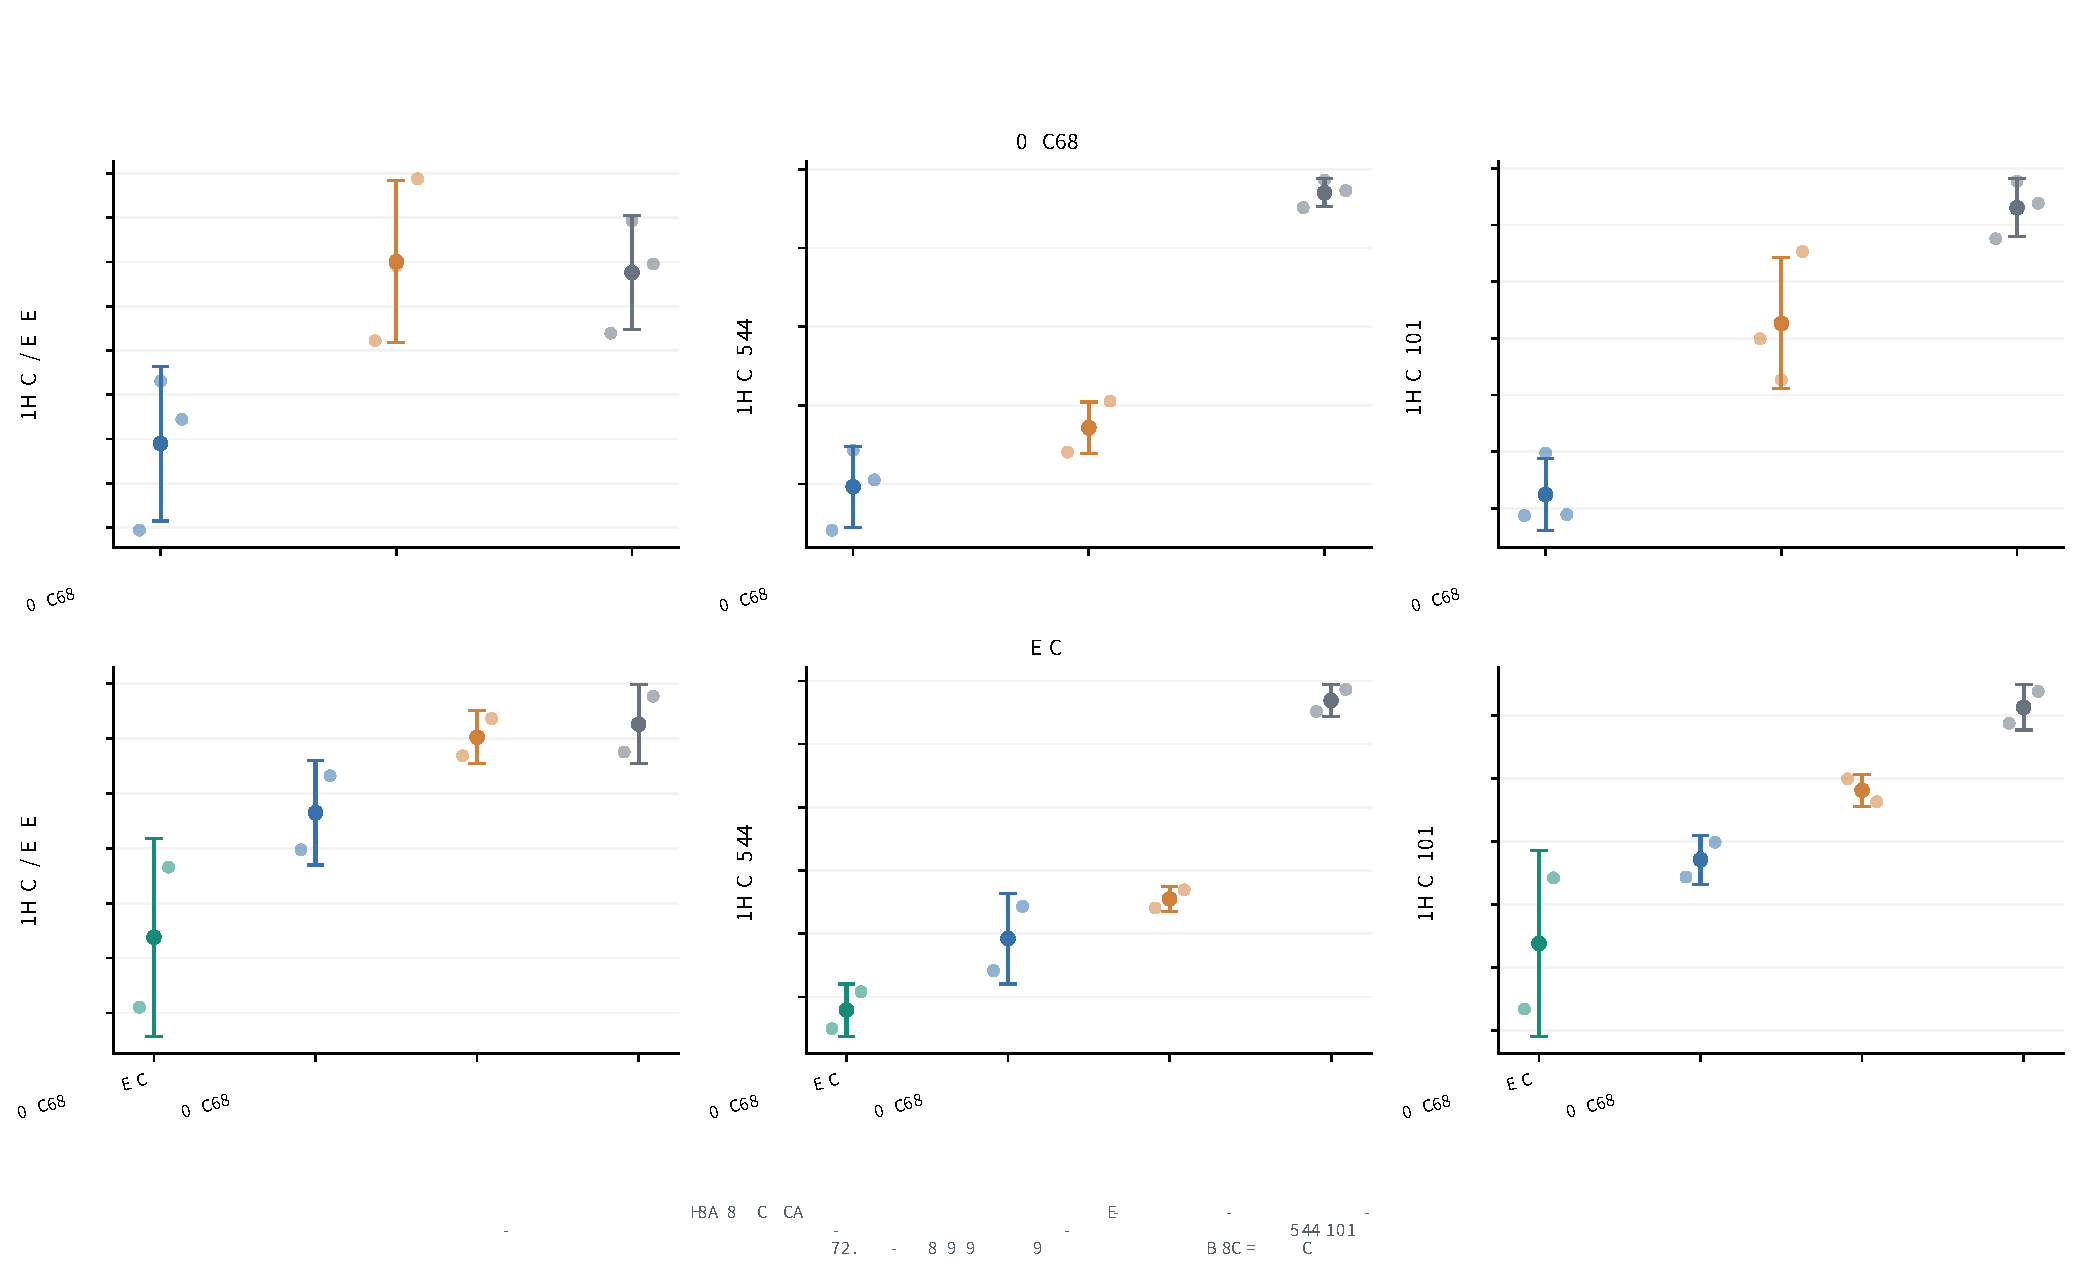
\includegraphics[width=.94\textwidth]{03_event_metrics.pdf}
\caption{Archived event metrics. Upper group: D1 three-seed original/independent/deterministic comparison. Lower group: D2 matched two-seed sampling exploration. Dots are individual seeds and bars are sample SD, not confidence intervals. Brier, NLL, ECE are separate event metrics. NLL/ECE are descriptive saved-prediction summaries.}
\end{figure}

\clearpage
\begin{figure}[H]\centering
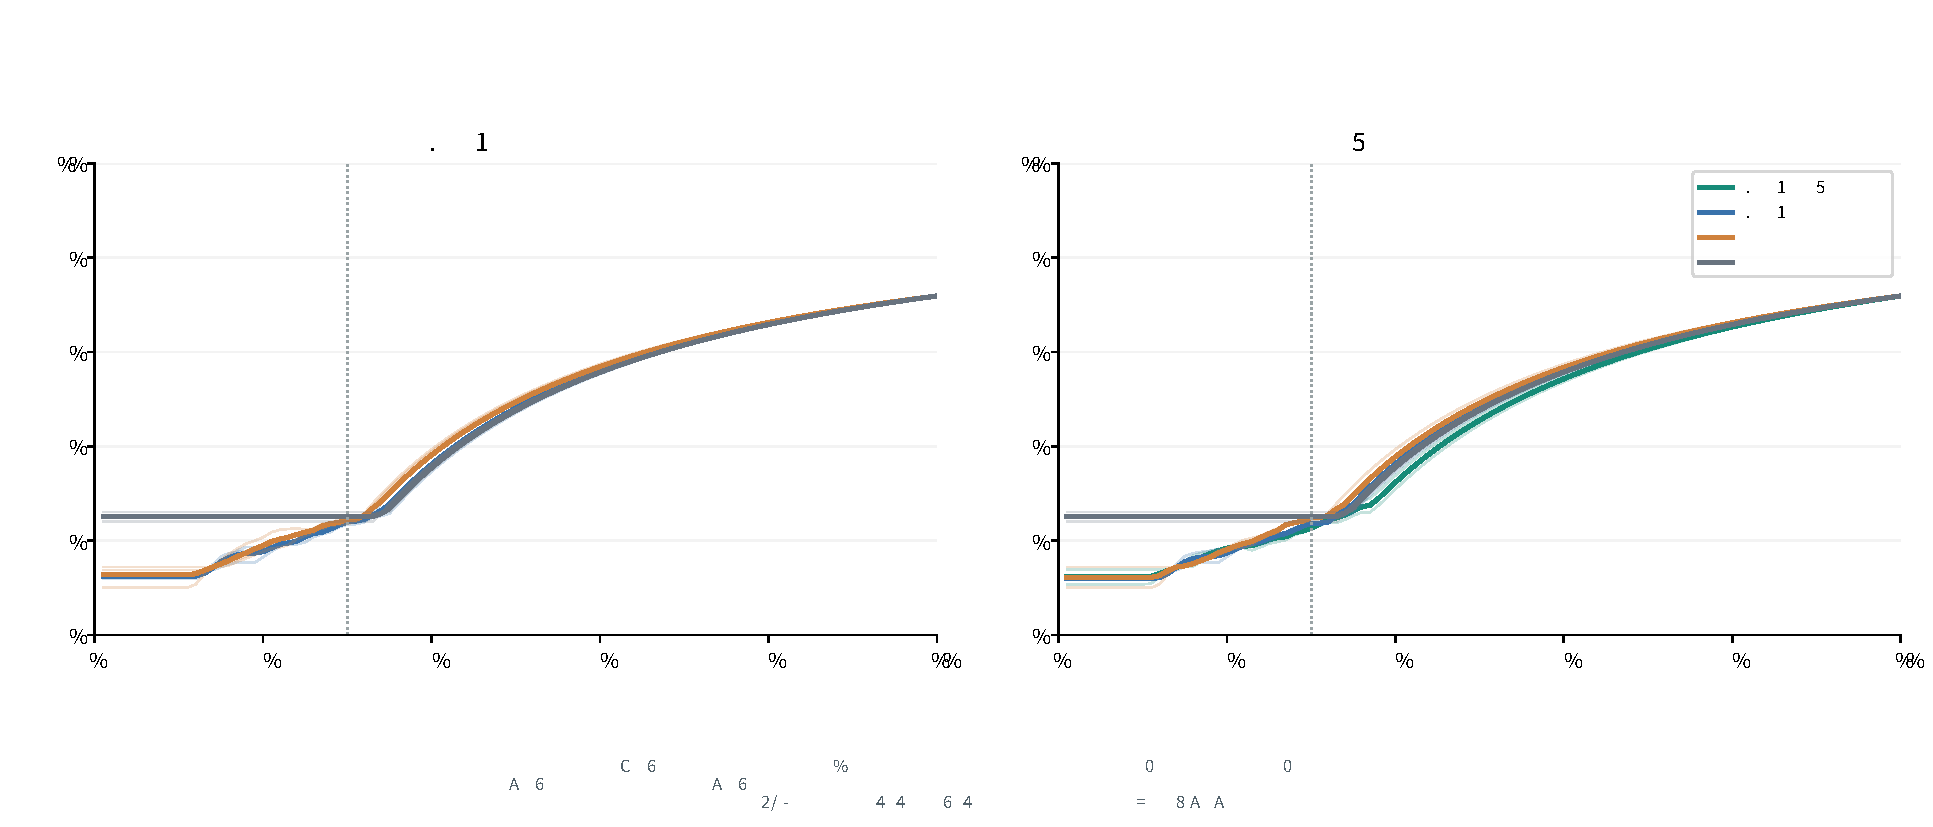
\includegraphics[width=.97\textwidth]{05_risk_coverage.pdf}
\caption{Archived selective risk versus weighted coverage. Thin curves denote seeds, thick curves their means. Boundary-score ties are accepted fractionally without labels. D1 and D2 remain separate groups. The horizontal axis is coverage, not confidence threshold; these curves do not establish a deployment safety guarantee.}
\end{figure}
\begin{figure}[H]\centering
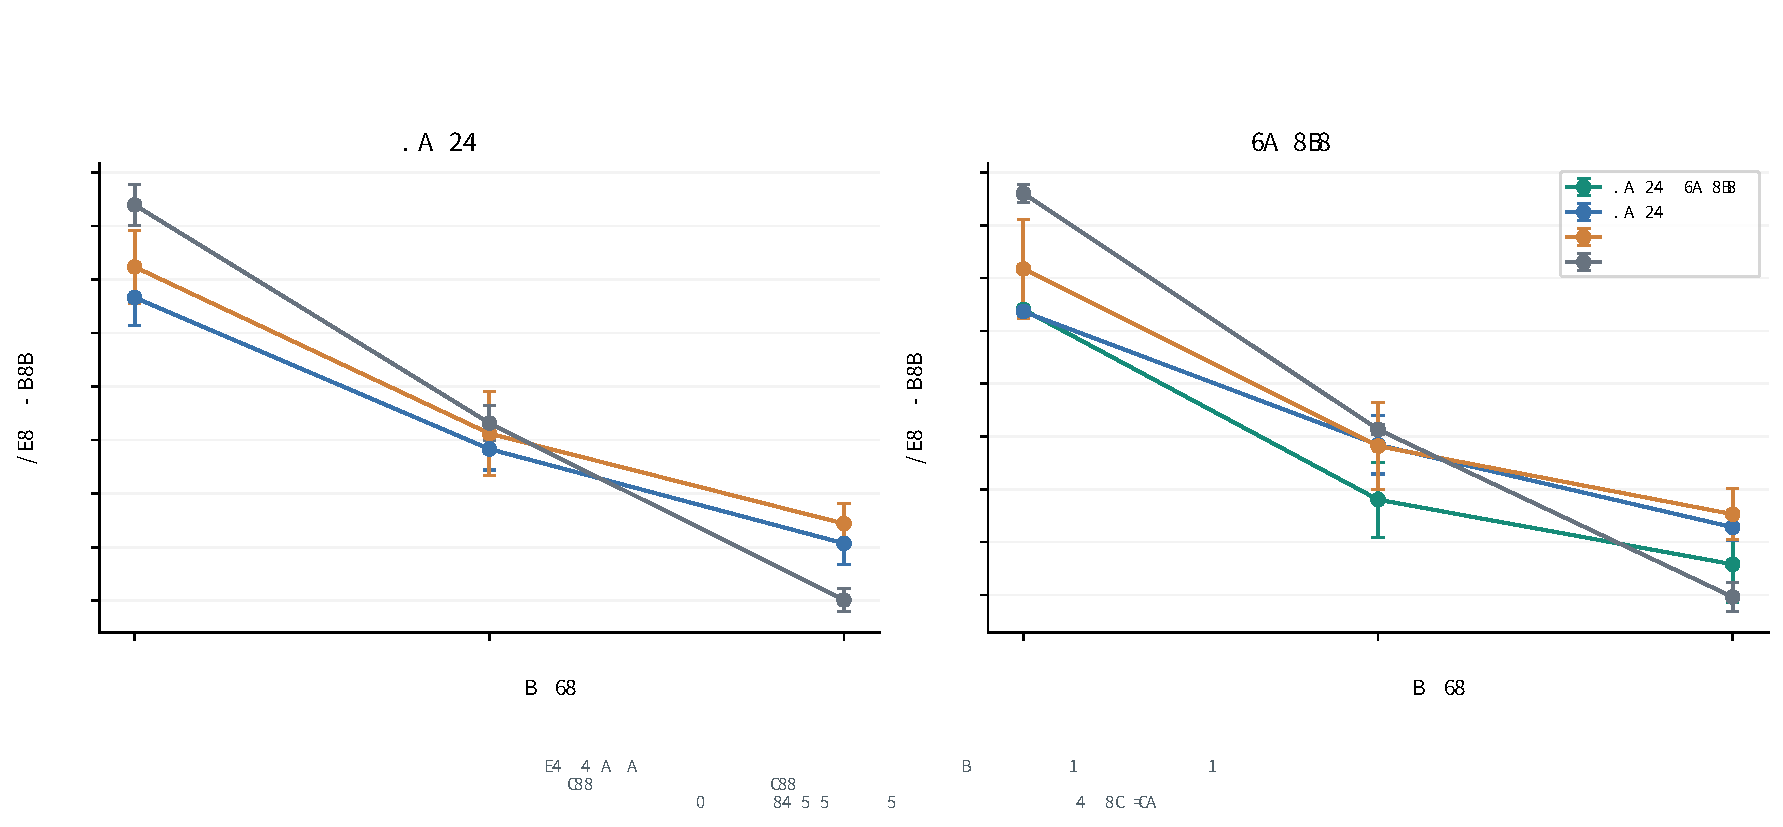
\includegraphics[width=.85\textwidth]{06_radius.pdf}
\caption{Archived Event Brier at frozen radii 0/10/20 cells. Error bars are training-seed SD and weights are recomputed within radius. Radius monotonicity of predictions does not imply uniformly better errors or meaningful acceptance for all radii; radius-20 ConPath threshold coverage is zero.}
\end{figure}

\clearpage
\begin{figure}[H]\centering
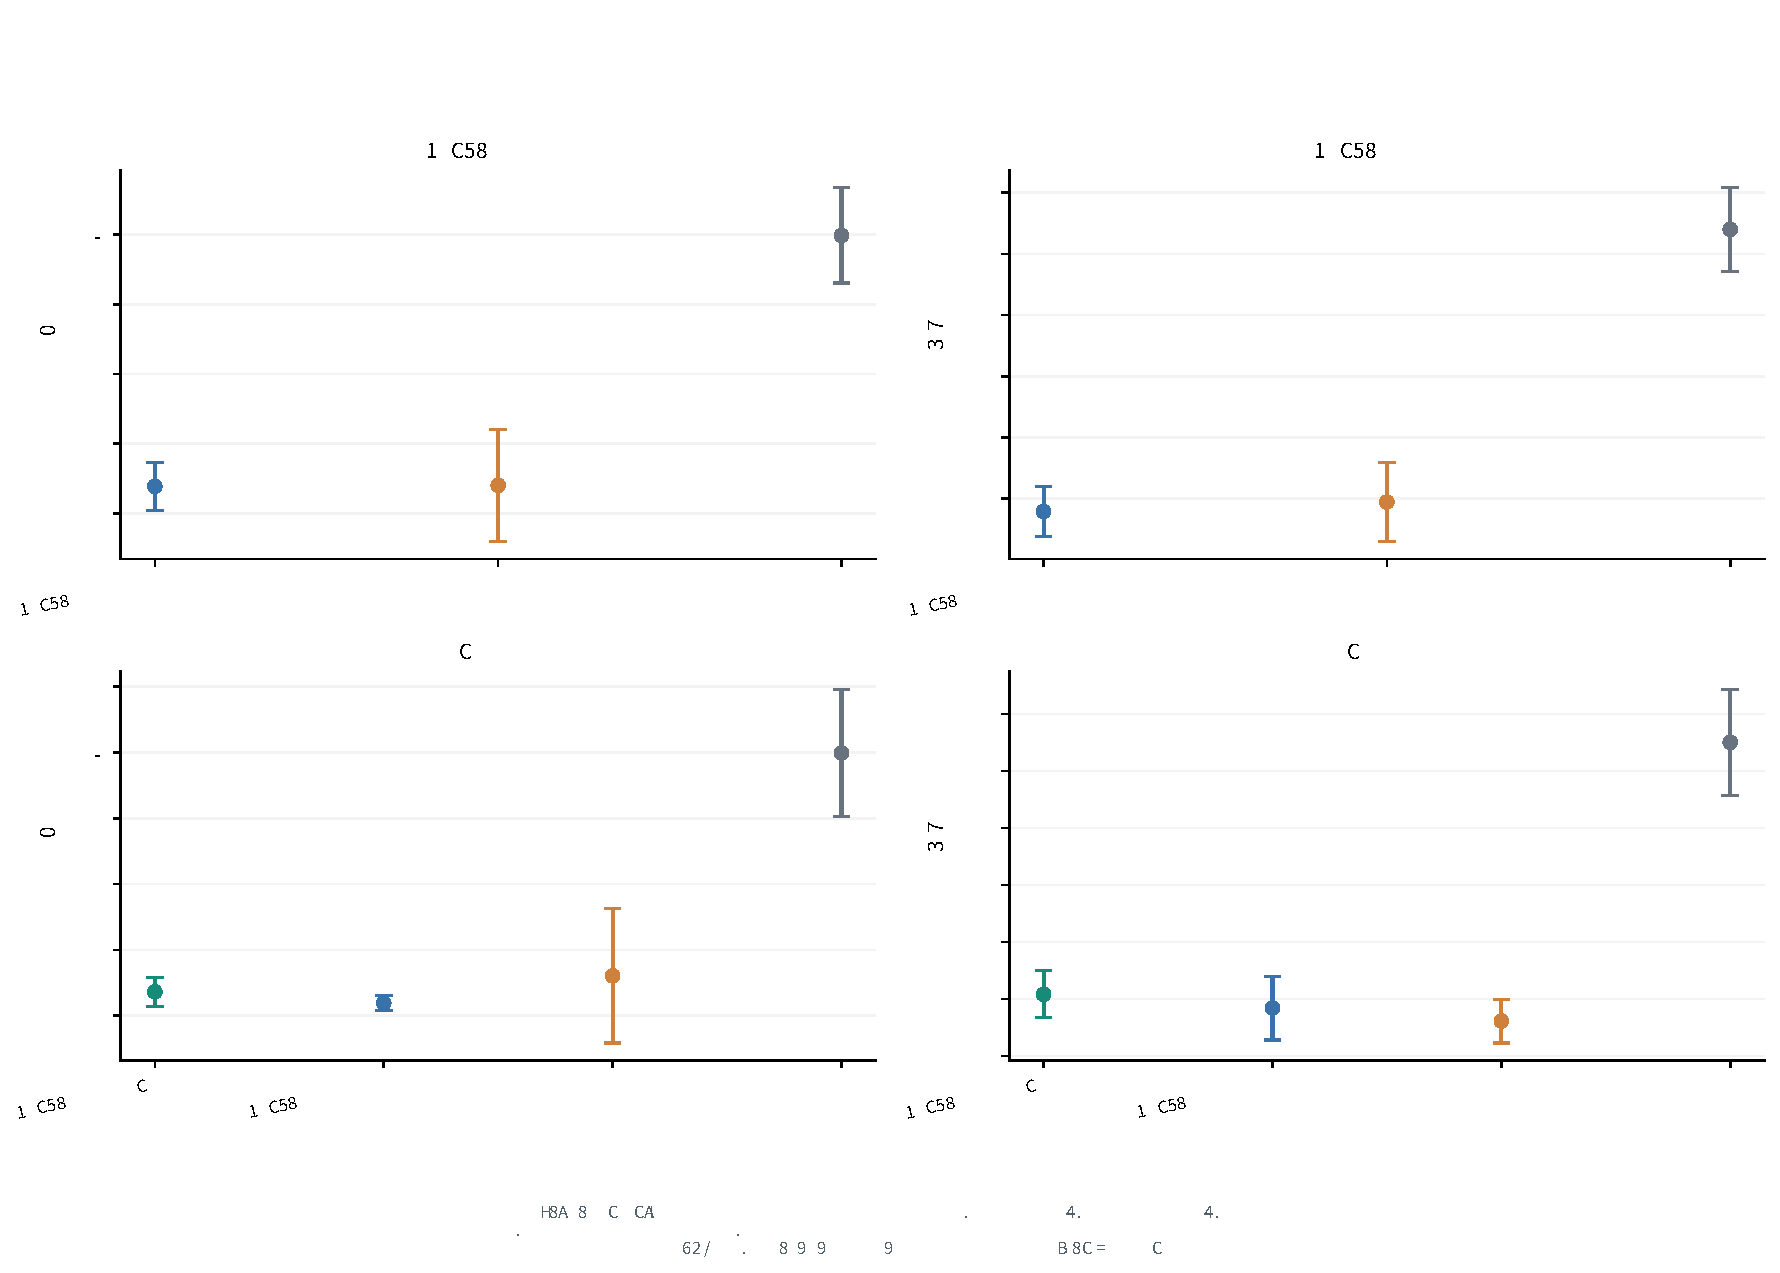
\includegraphics[width=.92\textwidth]{07_map_metrics.pdf}
\caption{Archived hidden valid-cell map diagnostics, separate from path-event scores. Empirical cell free frequency is not a path probability. Continuous deterministic map Brier is better than ConPath, as retained in the numerical tables; a binary-map score must not replace it.}
\end{figure}
\begin{figure}[H]\centering
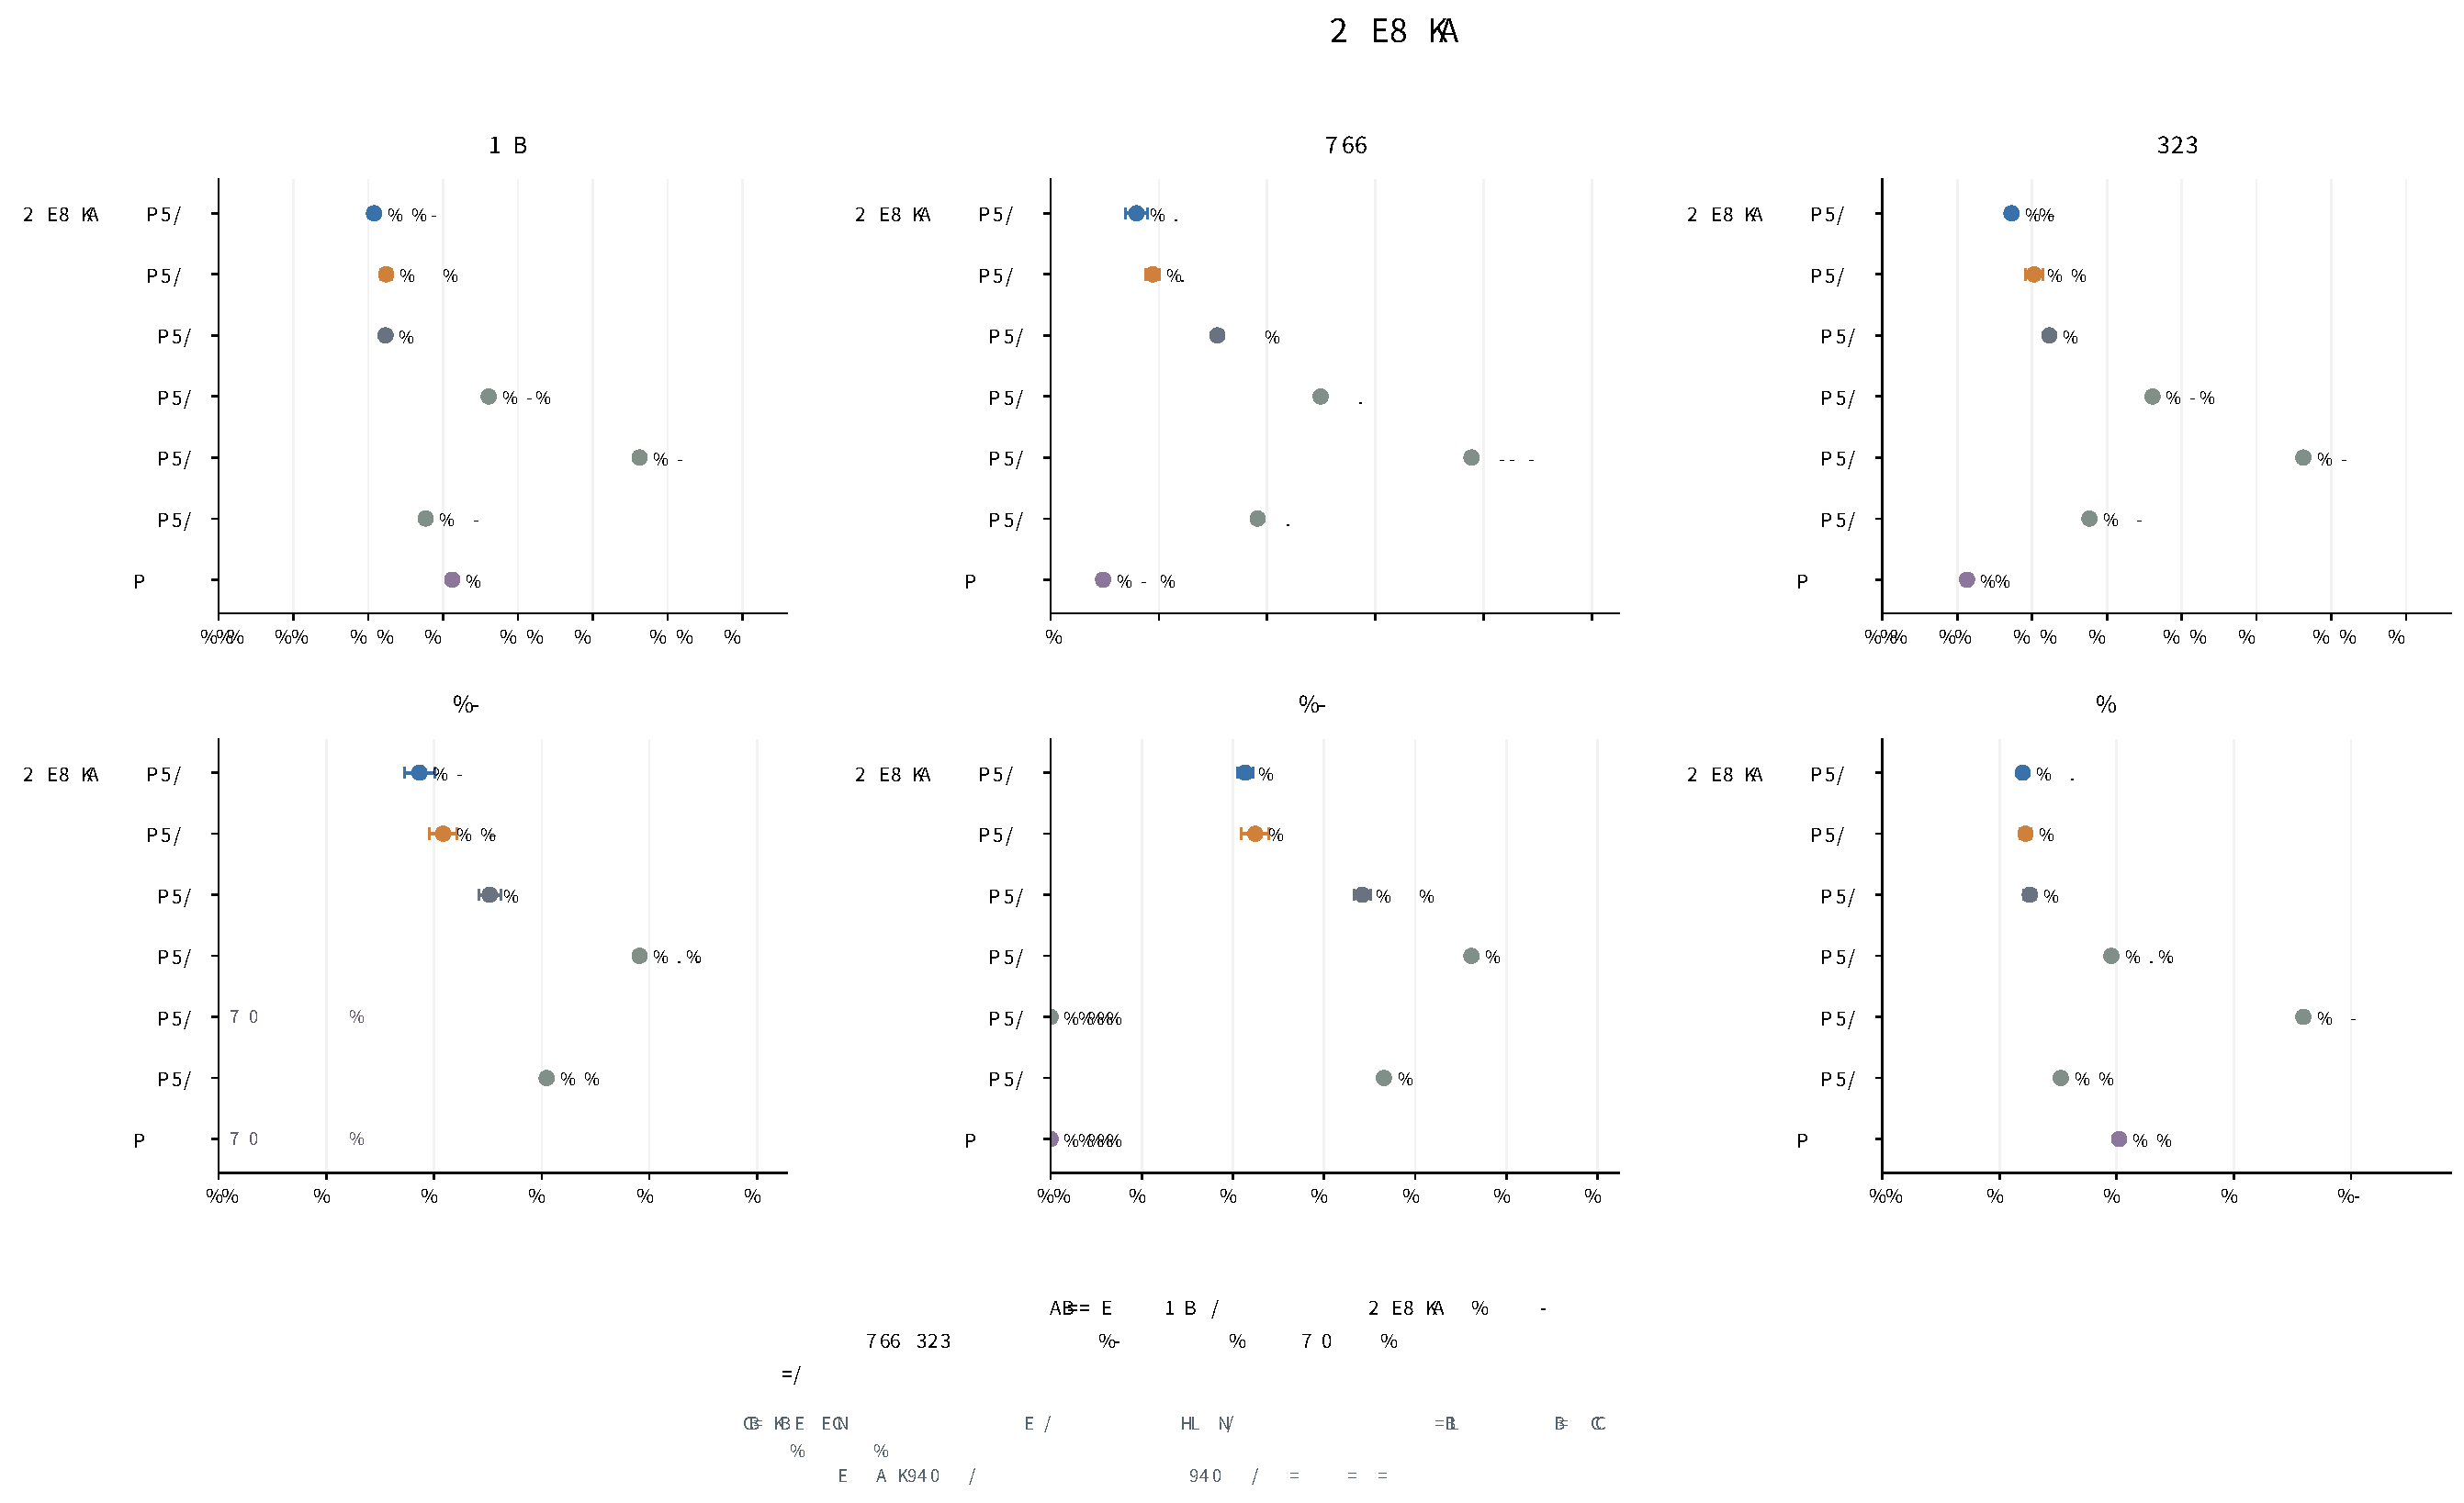
\includegraphics[width=.88\textwidth]{09_rule_controls.pdf}
\caption{All available D1 rule controls and trained methods. Rules are single deterministic evaluations, not three trained repeats. Undefined risk at zero coverage is omitted, not drawn as zero. The radius prior has lower NLL/ECE than ConPath but zero threshold-0.8 coverage. No method dominates all objectives.}
\end{figure}

\clearpage
\section{Fixed Qualitative Gallery}
All ten queries in the pre-existing identifier-selected list are retained, including failures. Every panel uses the same input, reference, query, seed 20260910, and radius 10 cells, and shows the first four saved worlds in their stored order. Displayed event forecasts use all 32 worlds. Rows are original ConPath, independent, and the separately trained D2 sampling candidate; the last is supplementary only. The maps are existing model samples, not hand-drawn completions.

\textbf{Legend for every case.} Green: free; dark: blocked; pale blue: valid unknown observation; checkerboard: invalid support, closed for connectivity. Blue circle S is start, orange diamond G is goal; rings show footprint extent. Columns are observed map, reference map, and four actual binary worlds. The reference is a label for evaluation, not an input to inference. No straight S--G segment is a predicted trajectory.

No strict interior-bottleneck example is available in this fixed set after requiring reference radius-0 reachability, current-radius unreachability, and both terminals fitting the footprint. We do not replace queries by outcome-selected cases. No complete preregistered occlusion sweep is available. The gallery therefore does not complete all of RQ3.
\begin{figure}[H]\centering
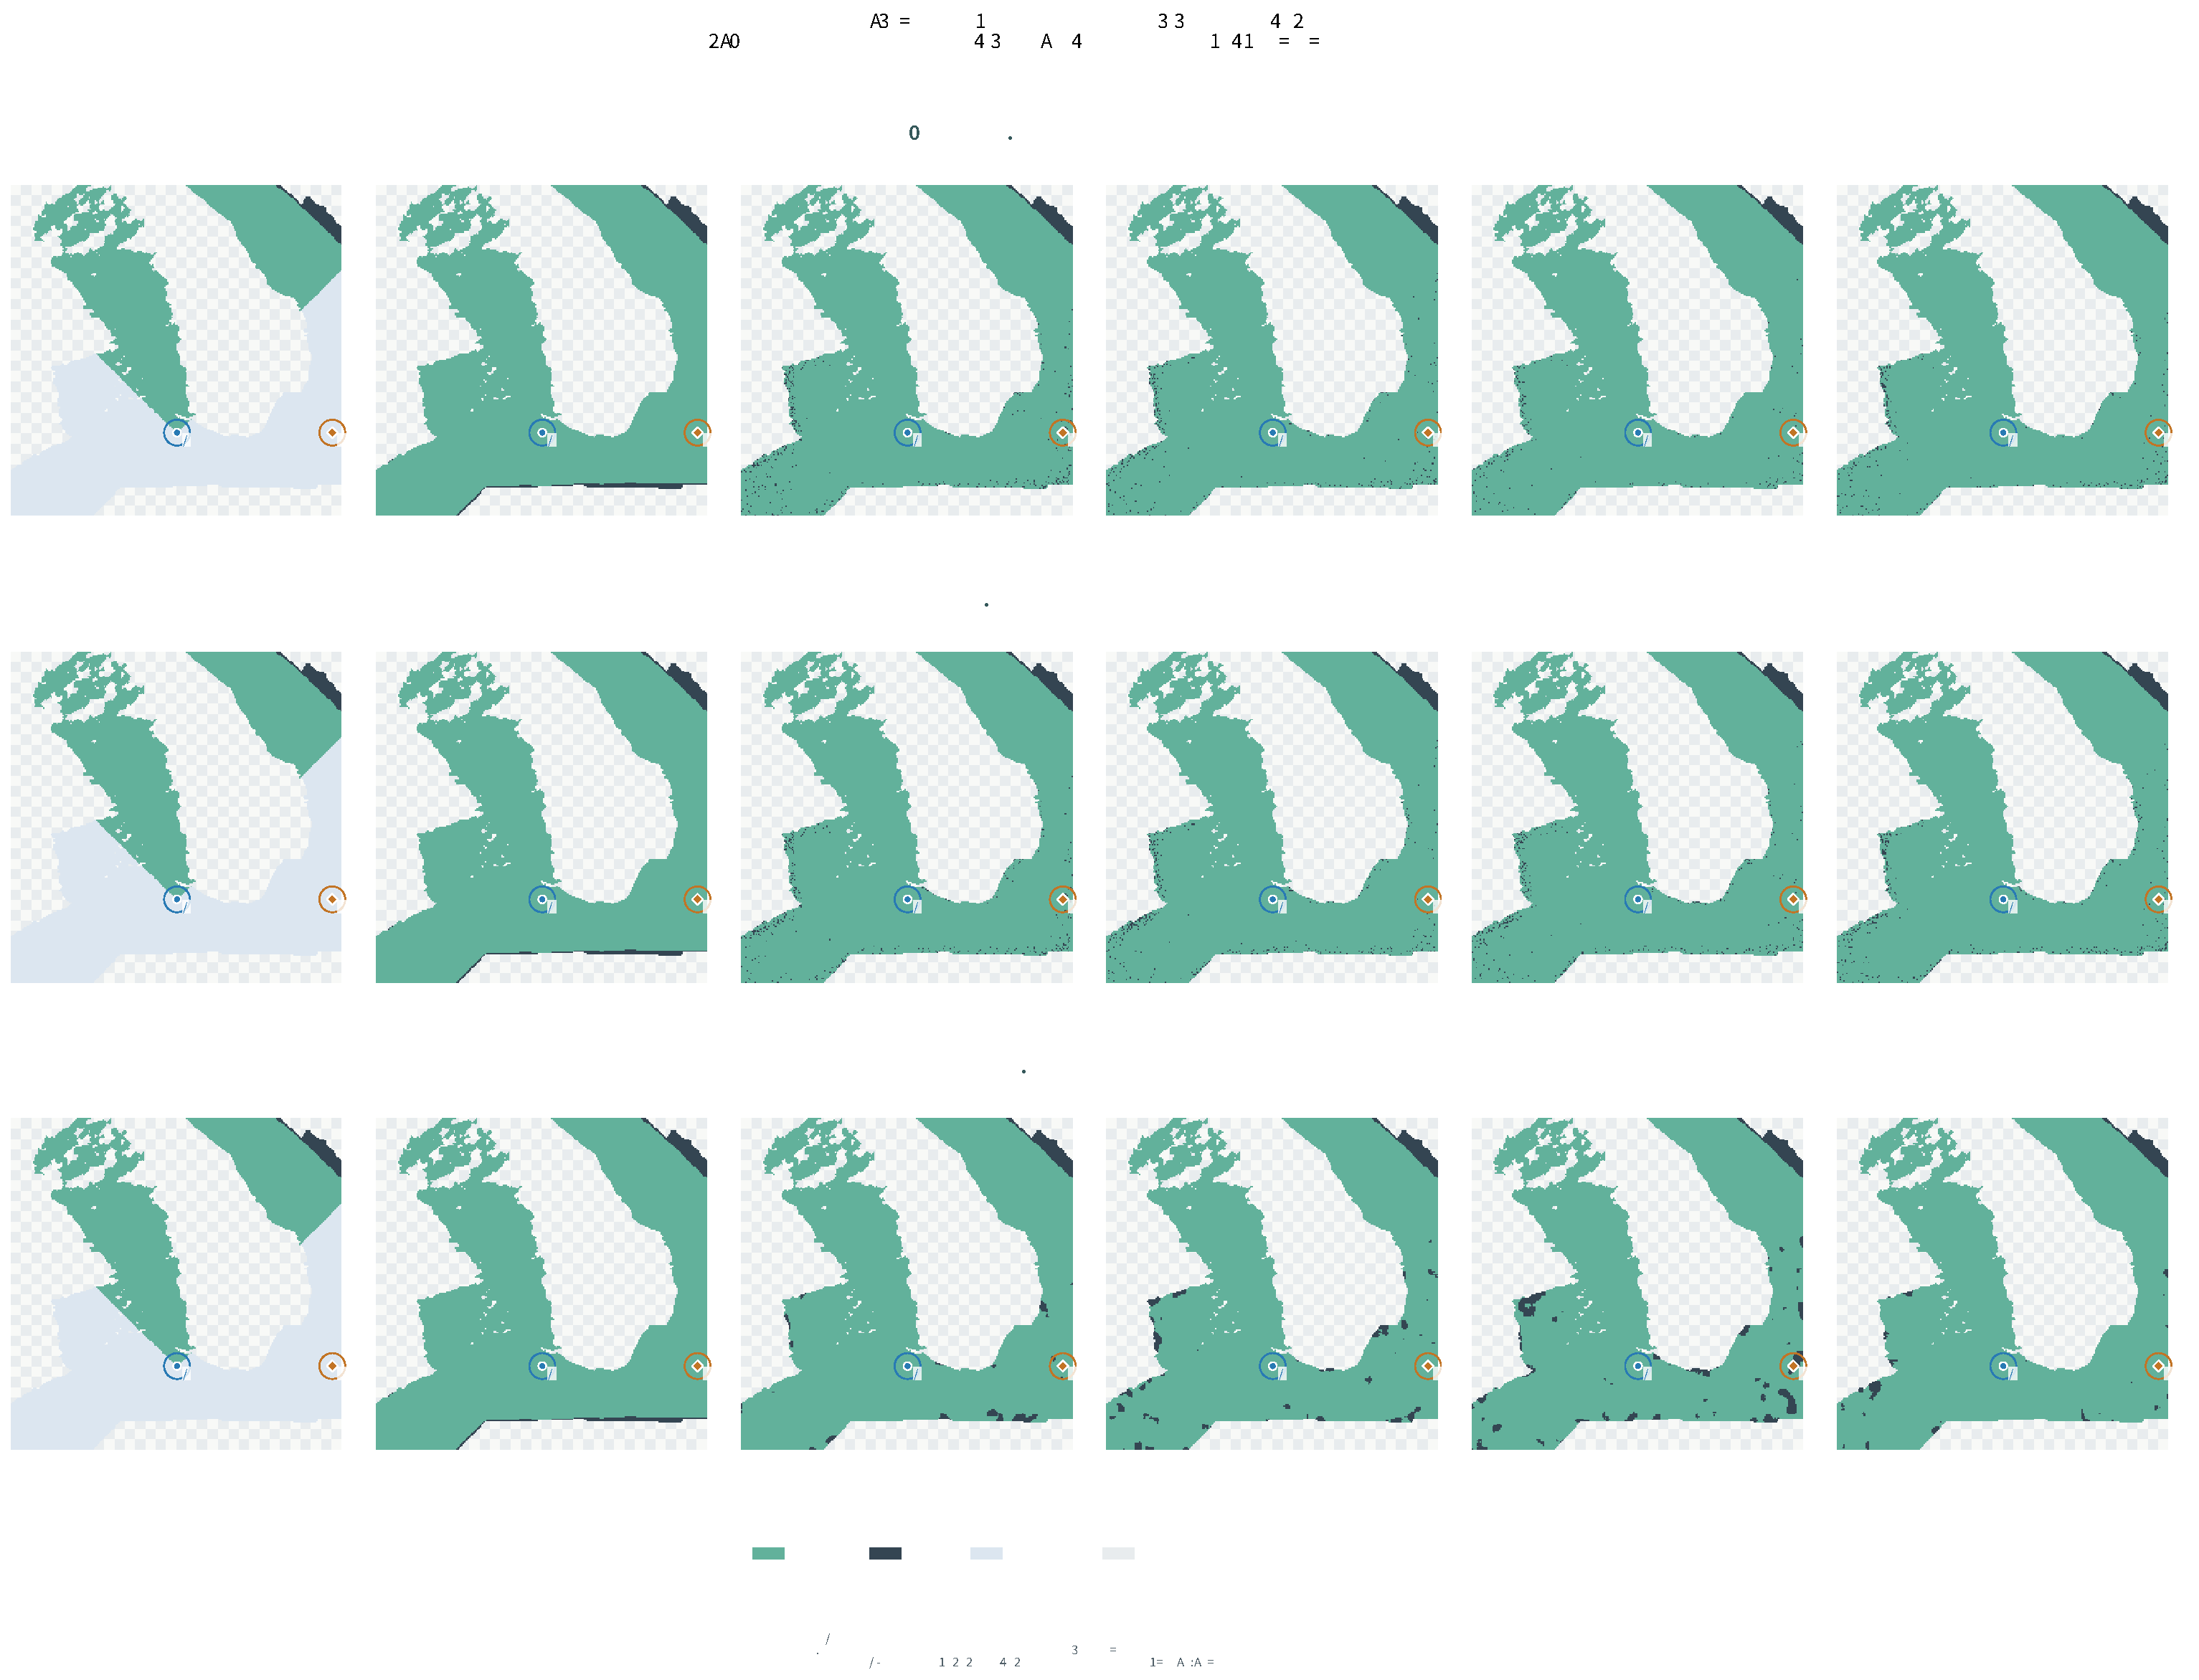
\includegraphics[width=.98\textwidth]{02_fixed_case_00.pdf}
\caption{Fixed archived gallery case 1: \texttt{obs\_014028:q024}, radius 10 grid cells, seed 20260910, validation-only. Same input and query across rows; first four stored worlds, with event frequencies from all 32. Original ConPath and independent are main development methods; the correlated categorical-noise variant is supplementary only. No outcome-based replacement or sample selection is performed.}
\end{figure}
\clearpage
\begin{figure}[H]\centering
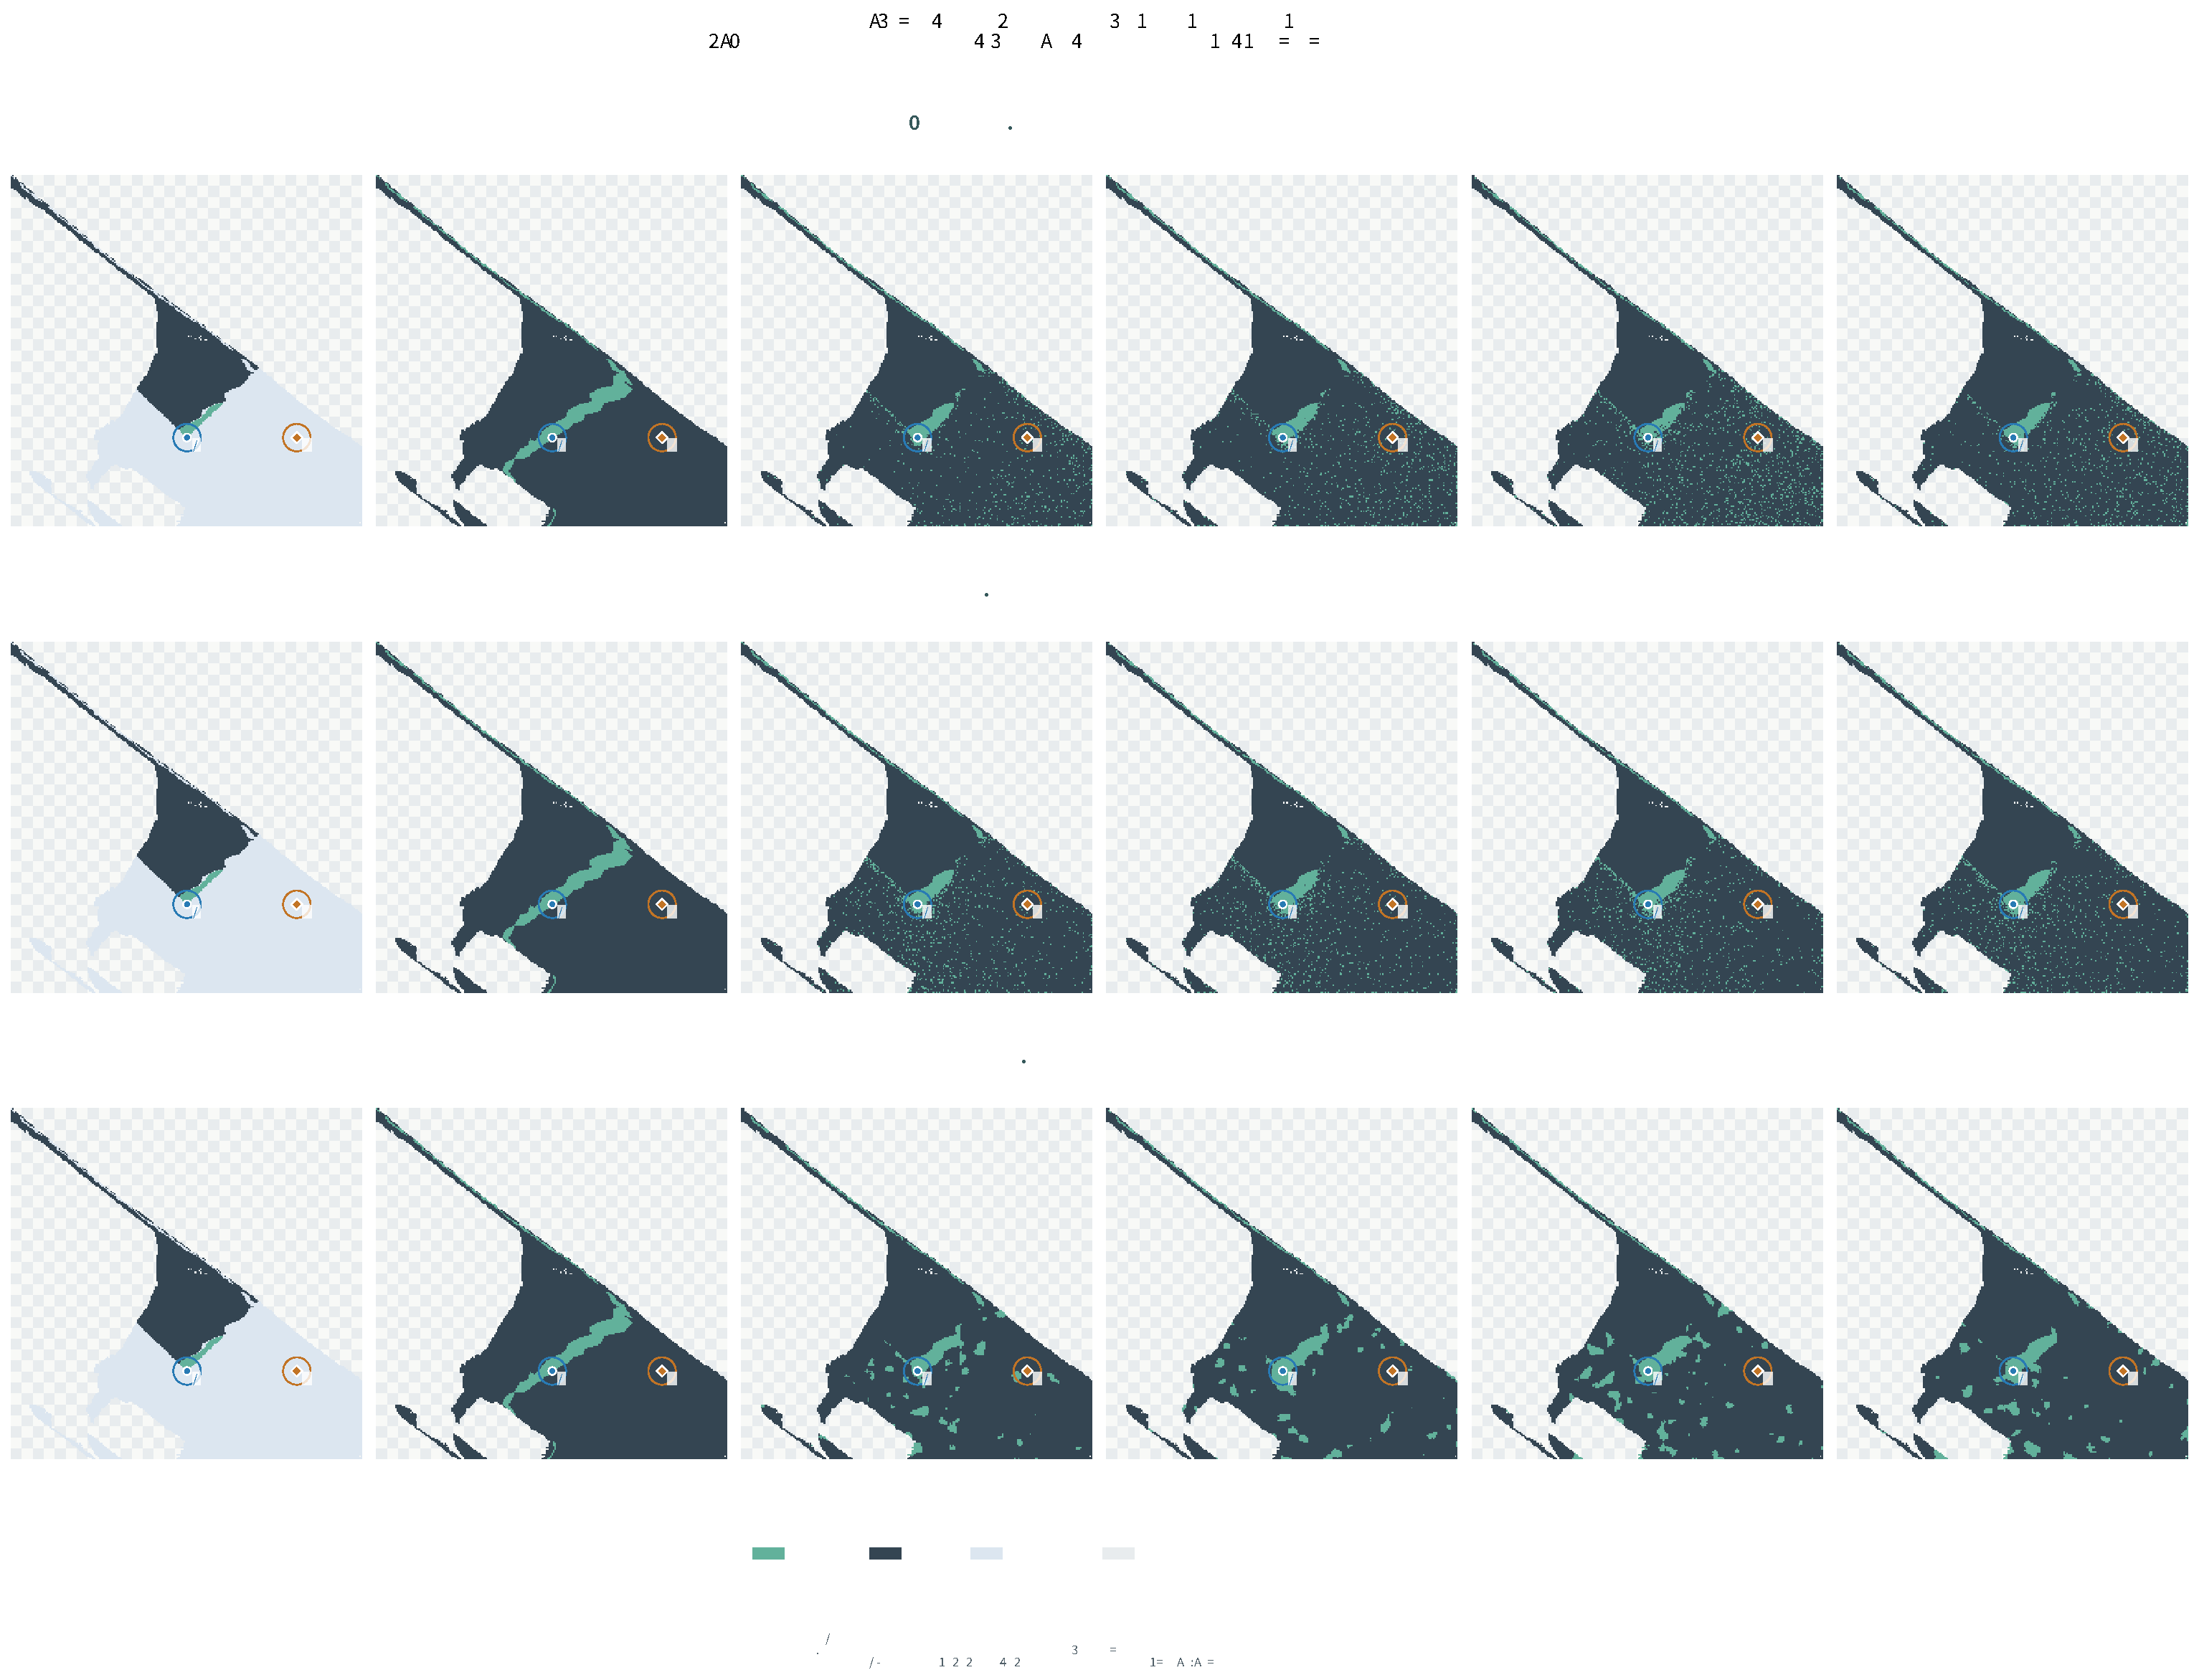
\includegraphics[width=.98\textwidth]{02_fixed_case_01.pdf}
\caption{Fixed archived gallery case 2: \texttt{obs\_013470:q012}, radius 10 grid cells, seed 20260910, validation-only. Same input and query across rows; first four stored worlds, with event frequencies from all 32. Original ConPath and independent are main development methods; the correlated categorical-noise variant is supplementary only. No outcome-based replacement or sample selection is performed.}
\end{figure}
\clearpage
\begin{figure}[H]\centering
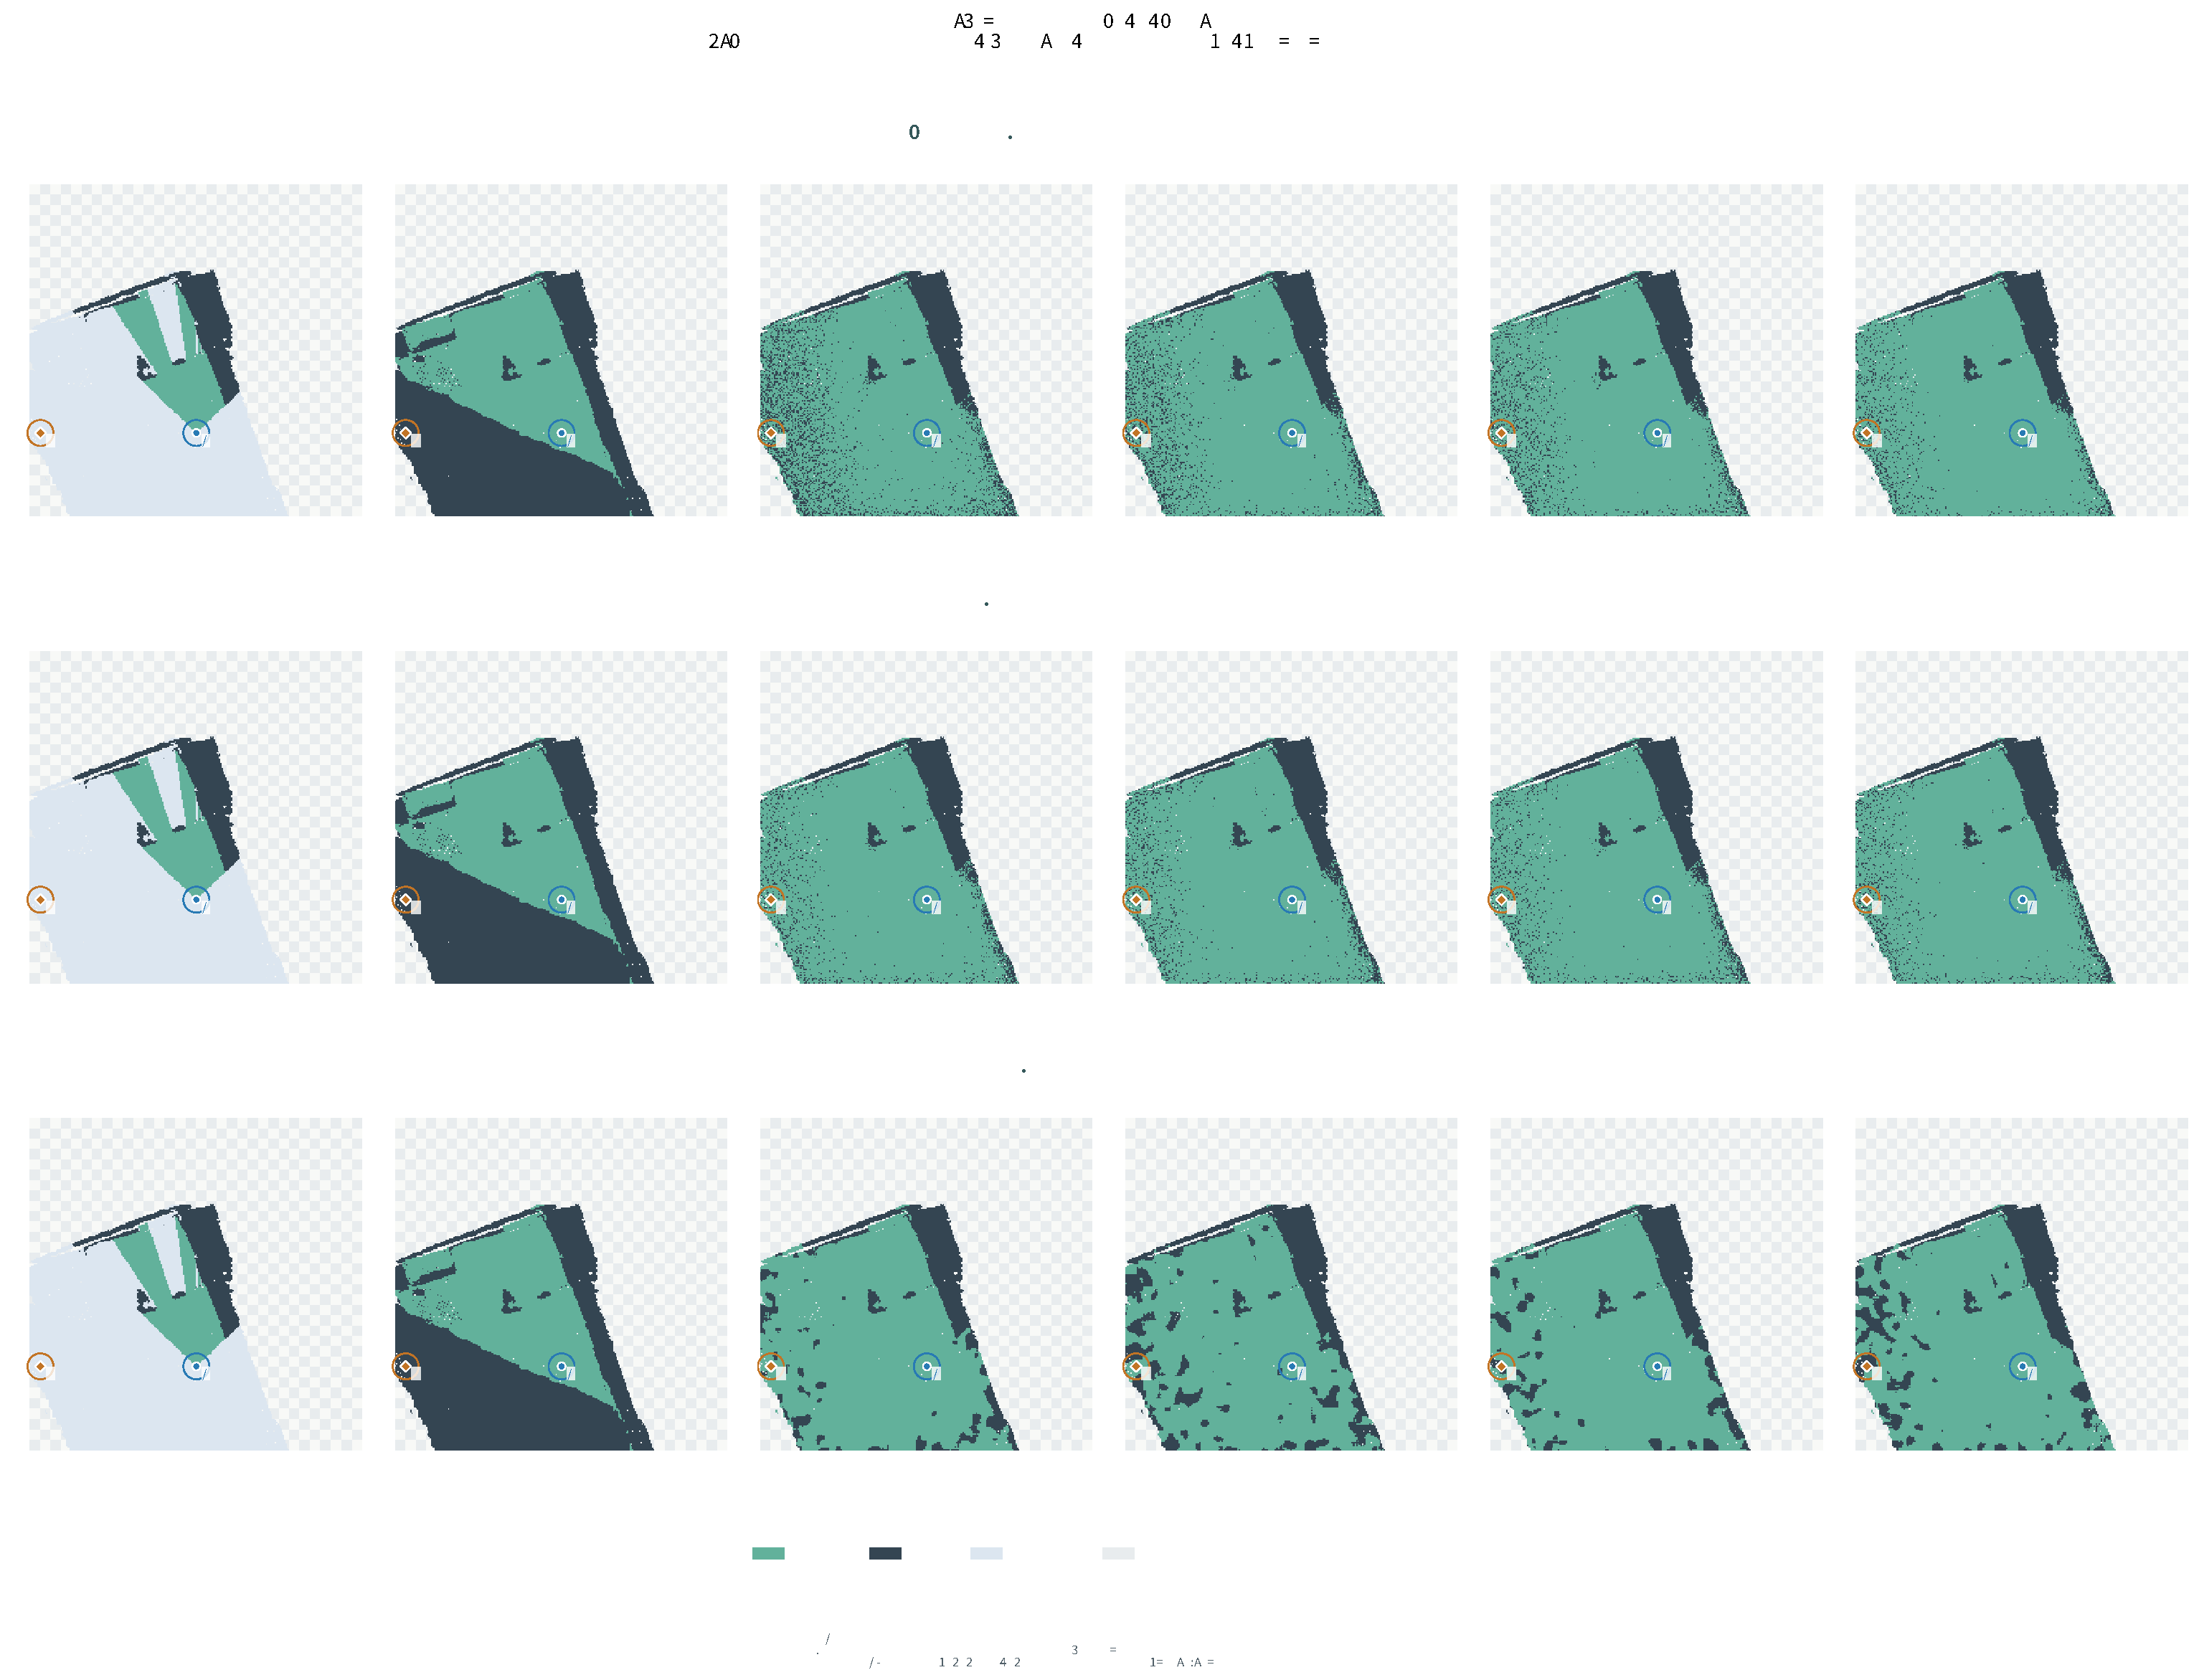
\includegraphics[width=.98\textwidth]{02_fixed_case_02.pdf}
\caption{Fixed archived gallery case 3: \texttt{obs\_082481:q030}, radius 10 grid cells, seed 20260910, validation-only. Same input and query across rows; first four stored worlds, with event frequencies from all 32. Original ConPath and independent are main development methods; the correlated categorical-noise variant is supplementary only. No outcome-based replacement or sample selection is performed.}
\end{figure}
\clearpage
\begin{figure}[H]\centering
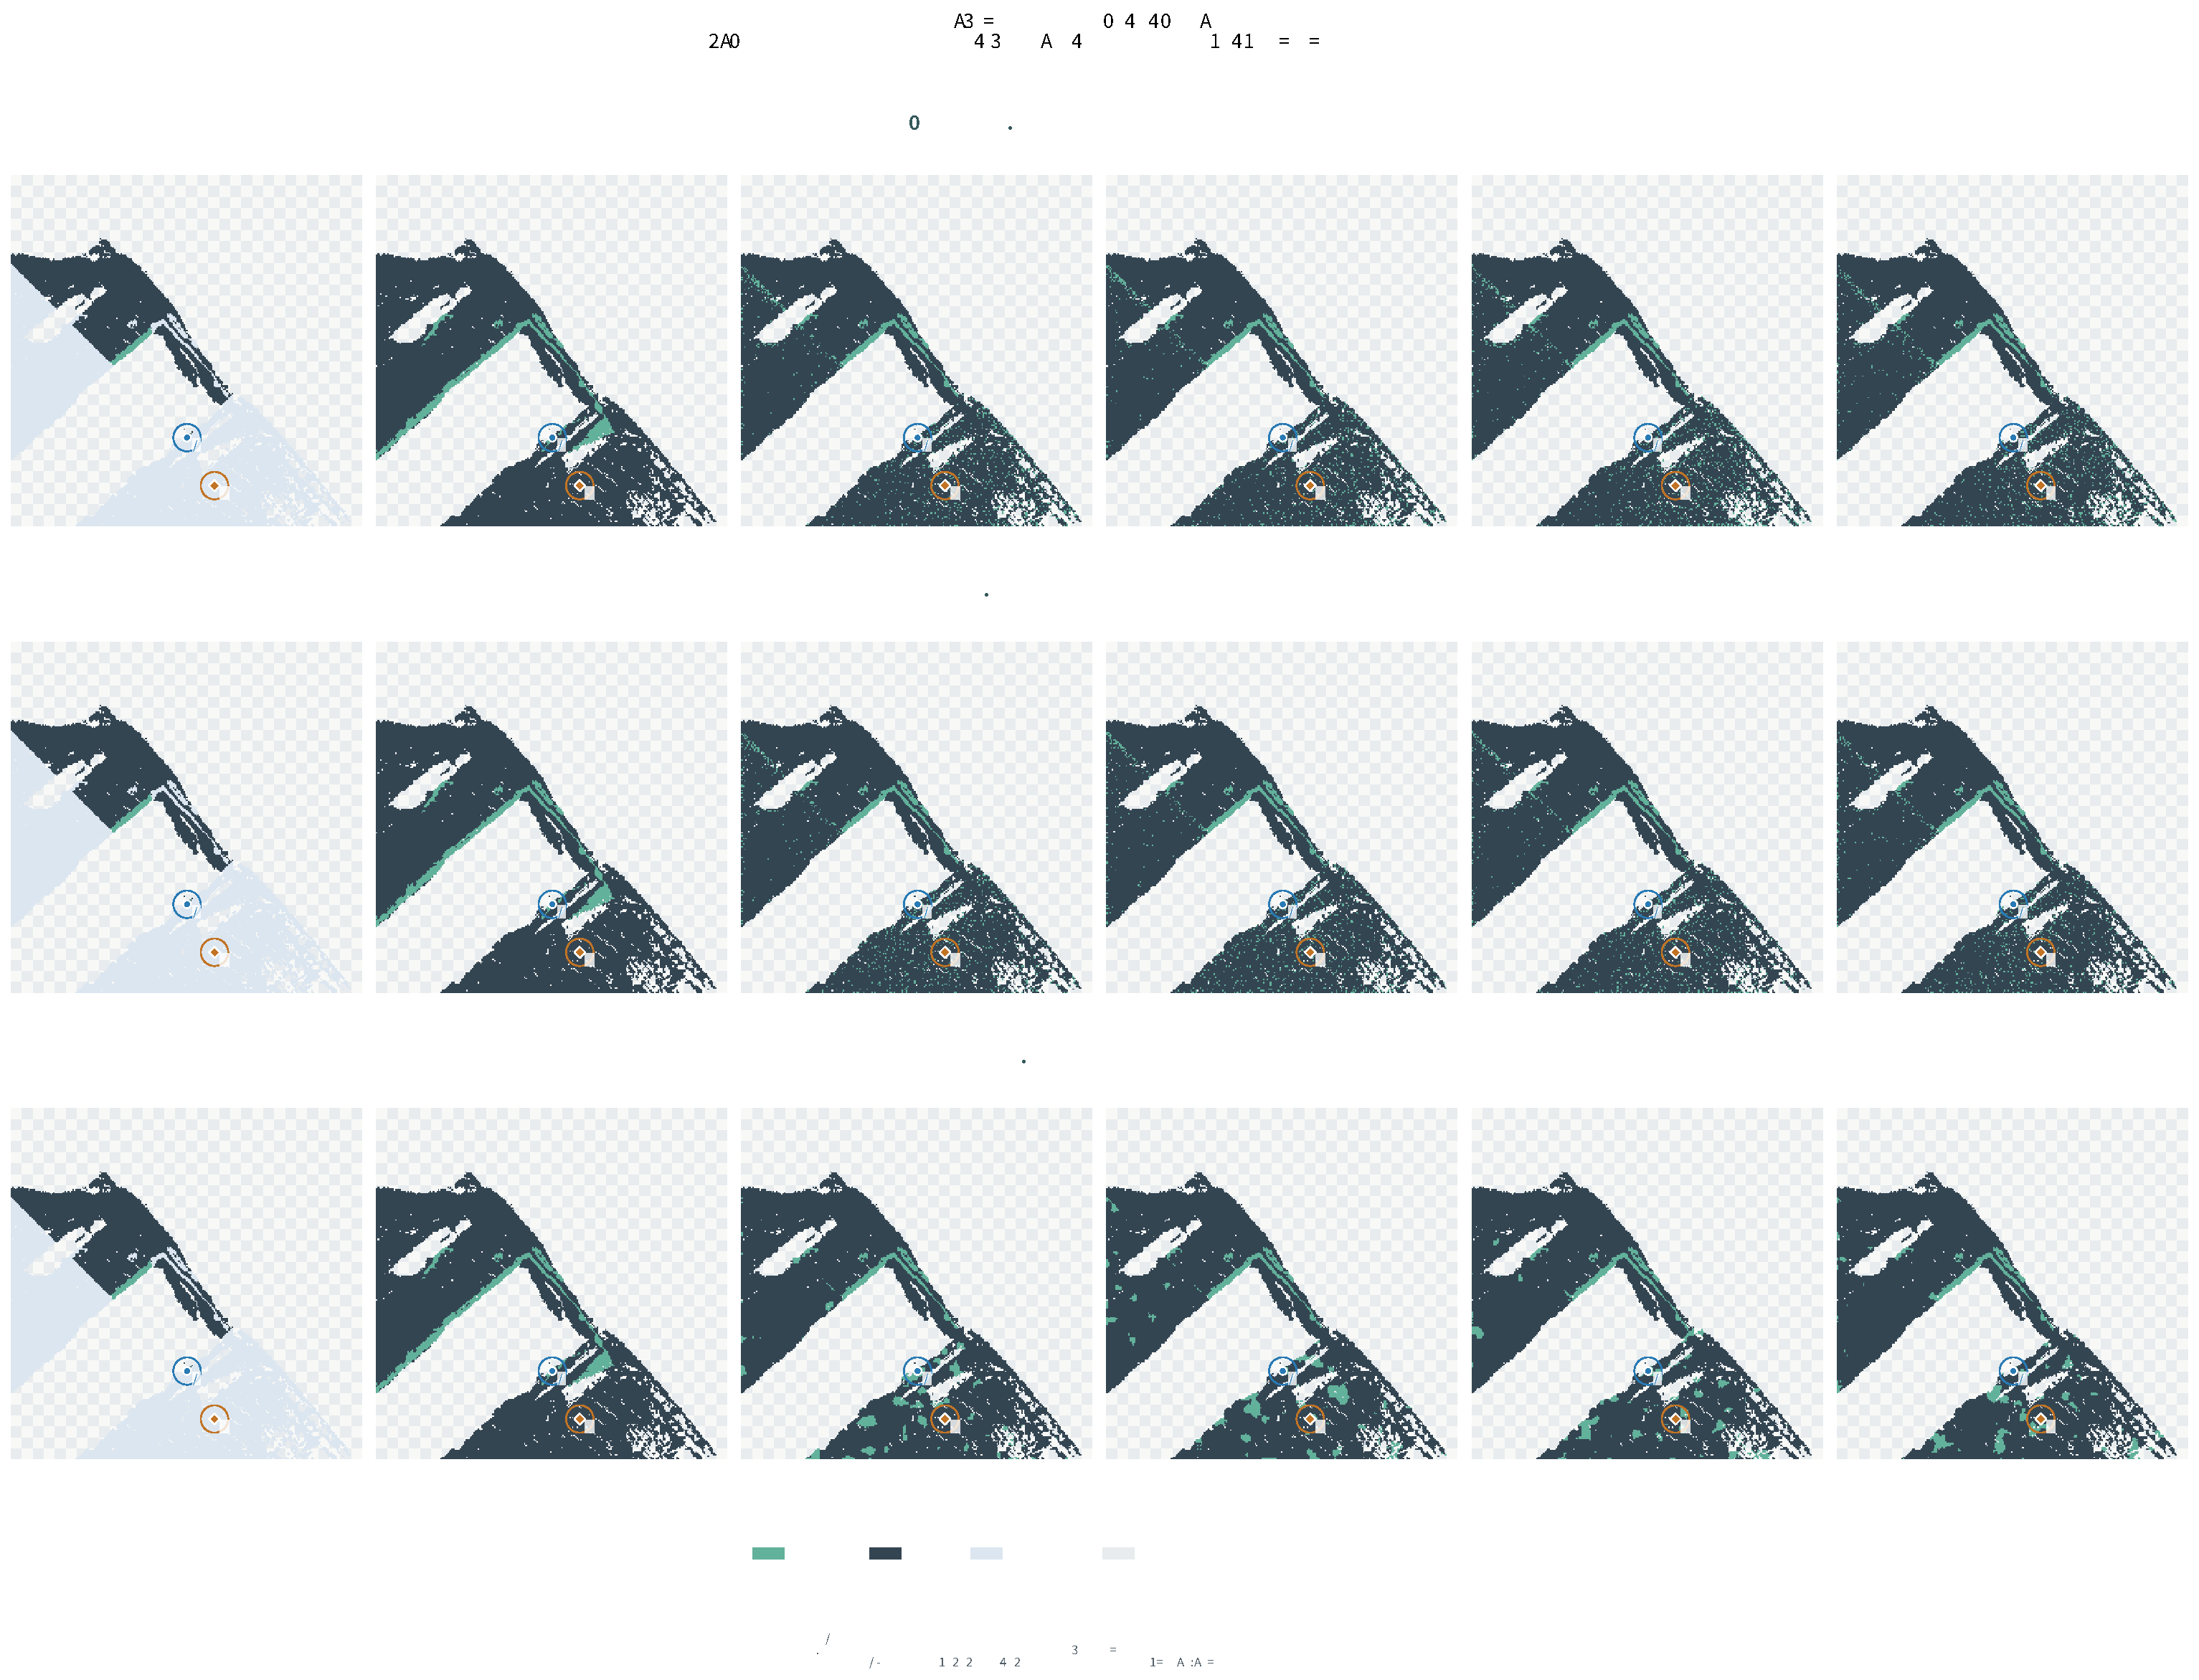
\includegraphics[width=.98\textwidth]{02_fixed_case_03.pdf}
\caption{Fixed archived gallery case 4: \texttt{obs\_065777:q002}, radius 10 grid cells, seed 20260910, validation-only. Same input and query across rows; first four stored worlds, with event frequencies from all 32. Original ConPath and independent are main development methods; the correlated categorical-noise variant is supplementary only. No outcome-based replacement or sample selection is performed.}
\end{figure}
\clearpage
\begin{figure}[H]\centering
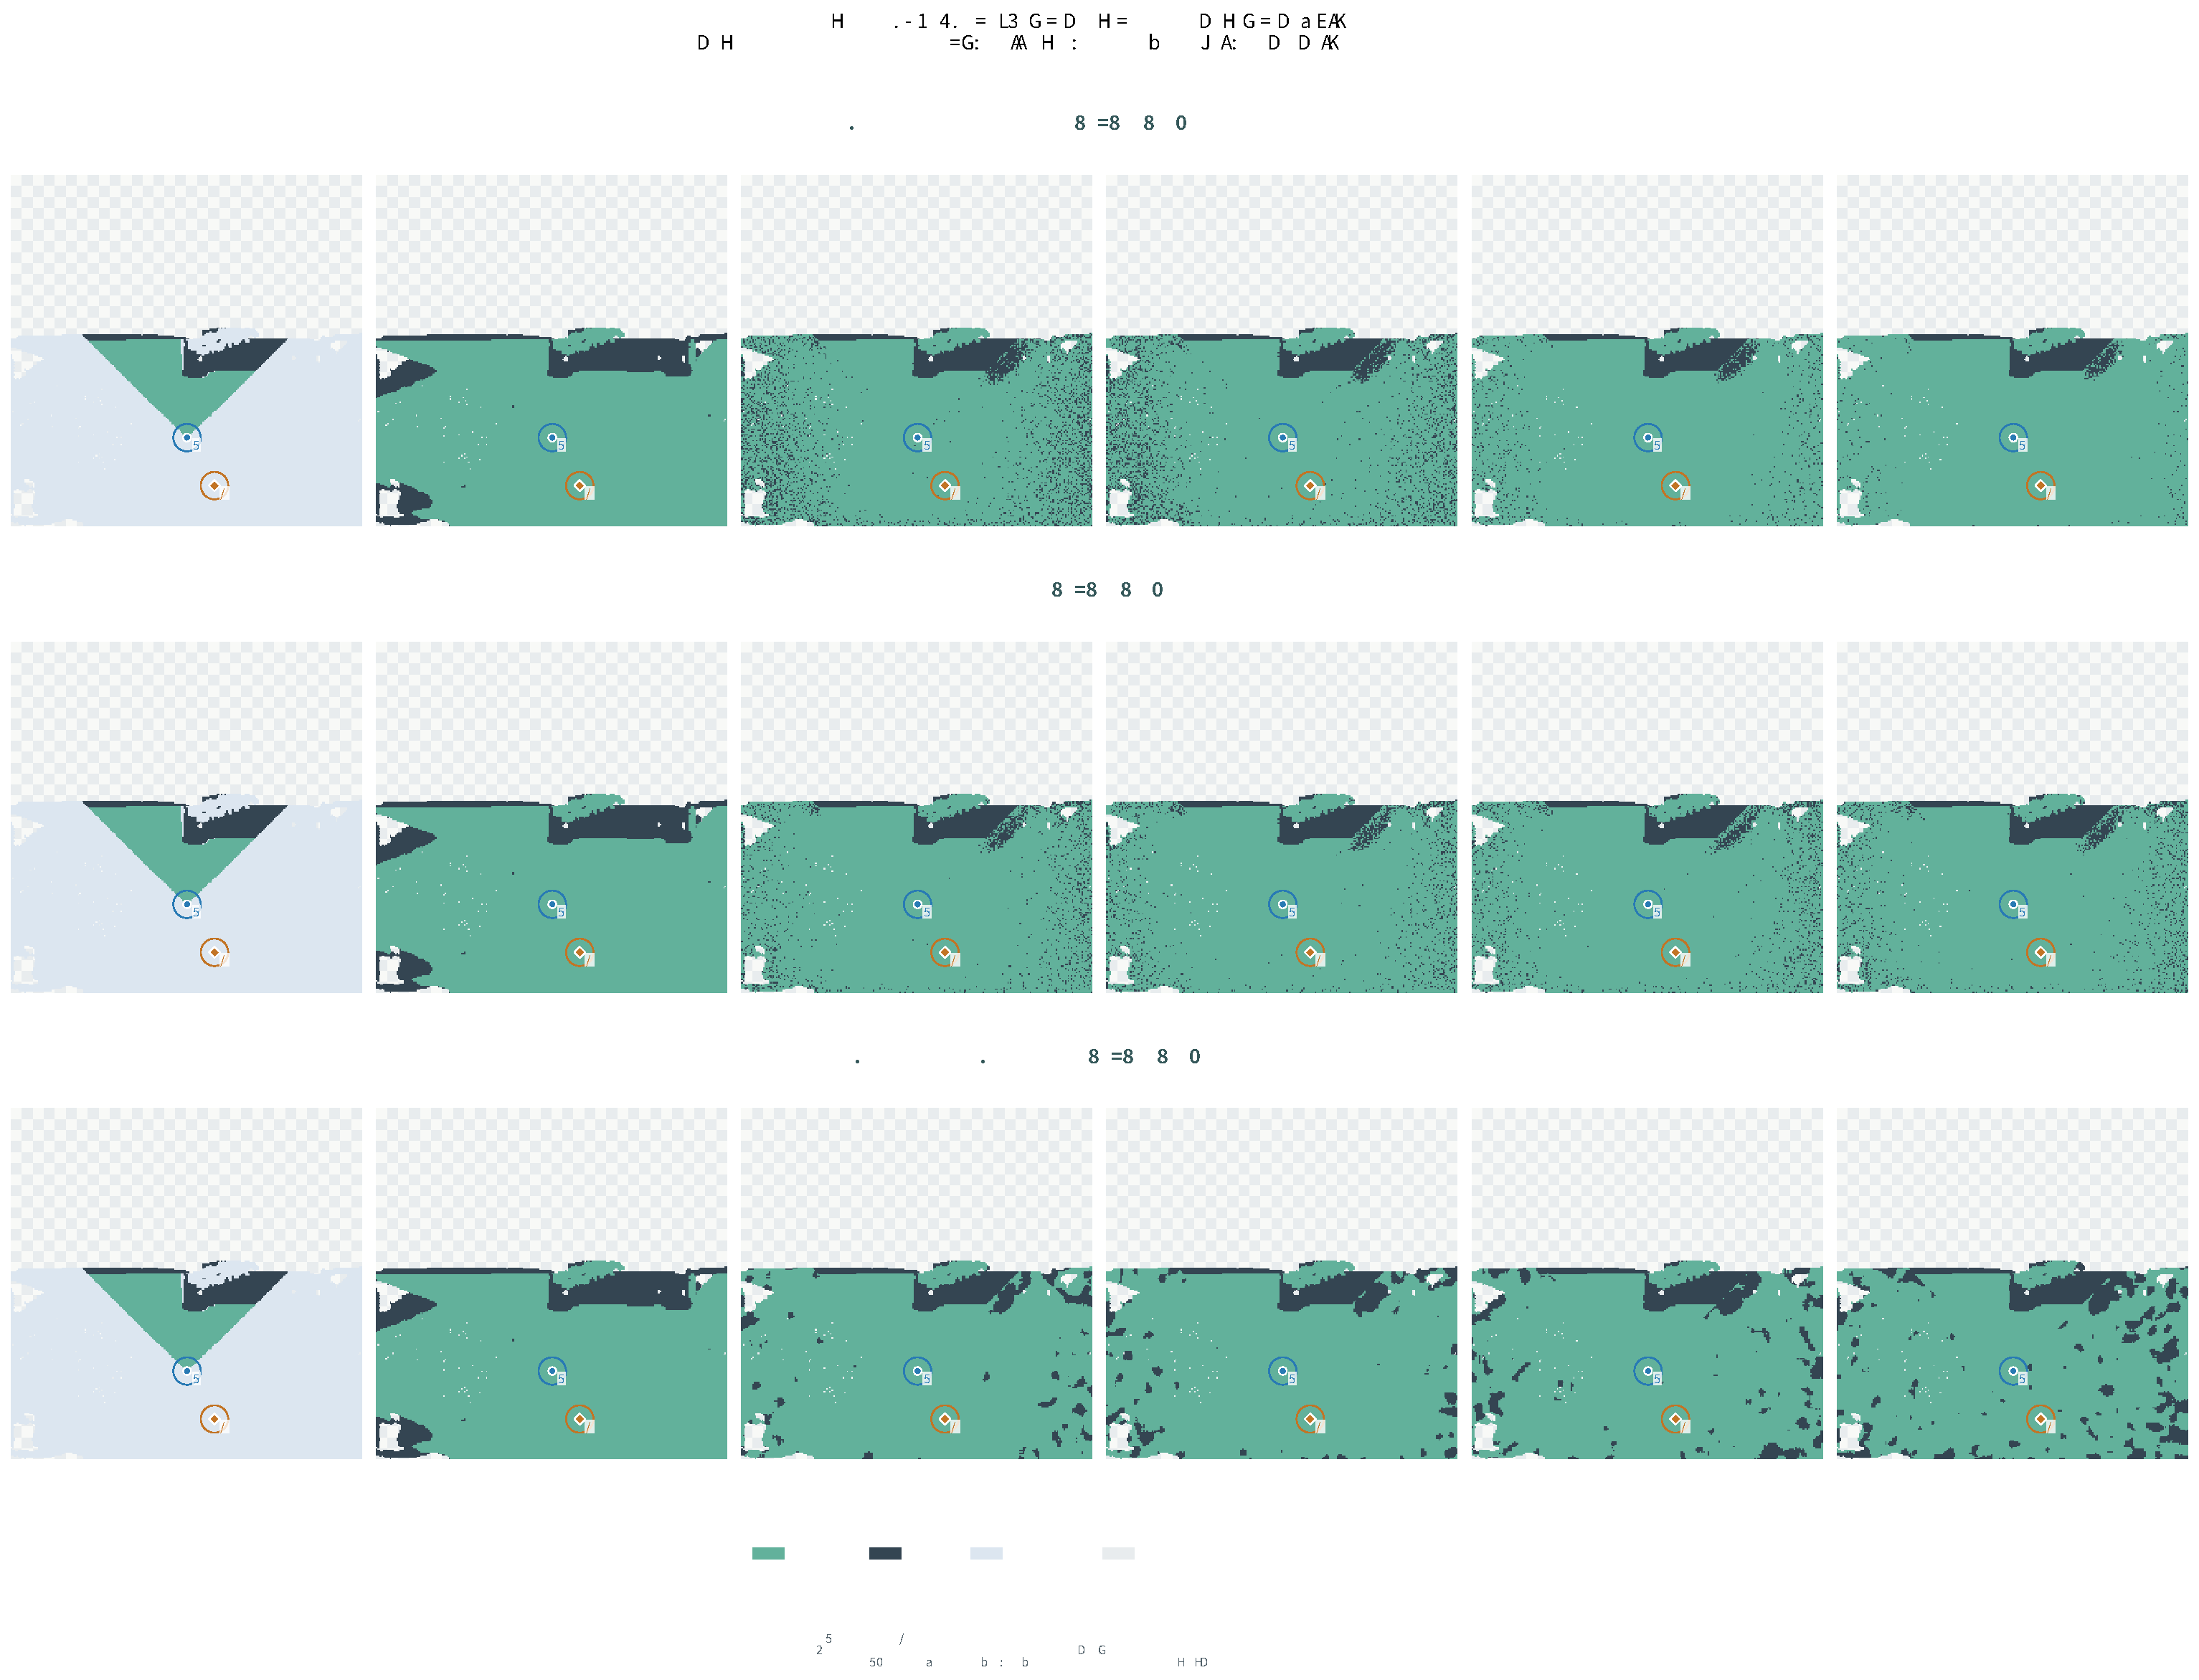
\includegraphics[width=.98\textwidth]{02_fixed_case_04.pdf}
\caption{Fixed archived gallery case 5: \texttt{obs\_114561:q002}, radius 10 grid cells, seed 20260910, validation-only. Same input and query across rows; first four stored worlds, with event frequencies from all 32. Original ConPath and independent are main development methods; the correlated categorical-noise variant is supplementary only. No outcome-based replacement or sample selection is performed.}
\end{figure}
\clearpage
\begin{figure}[H]\centering
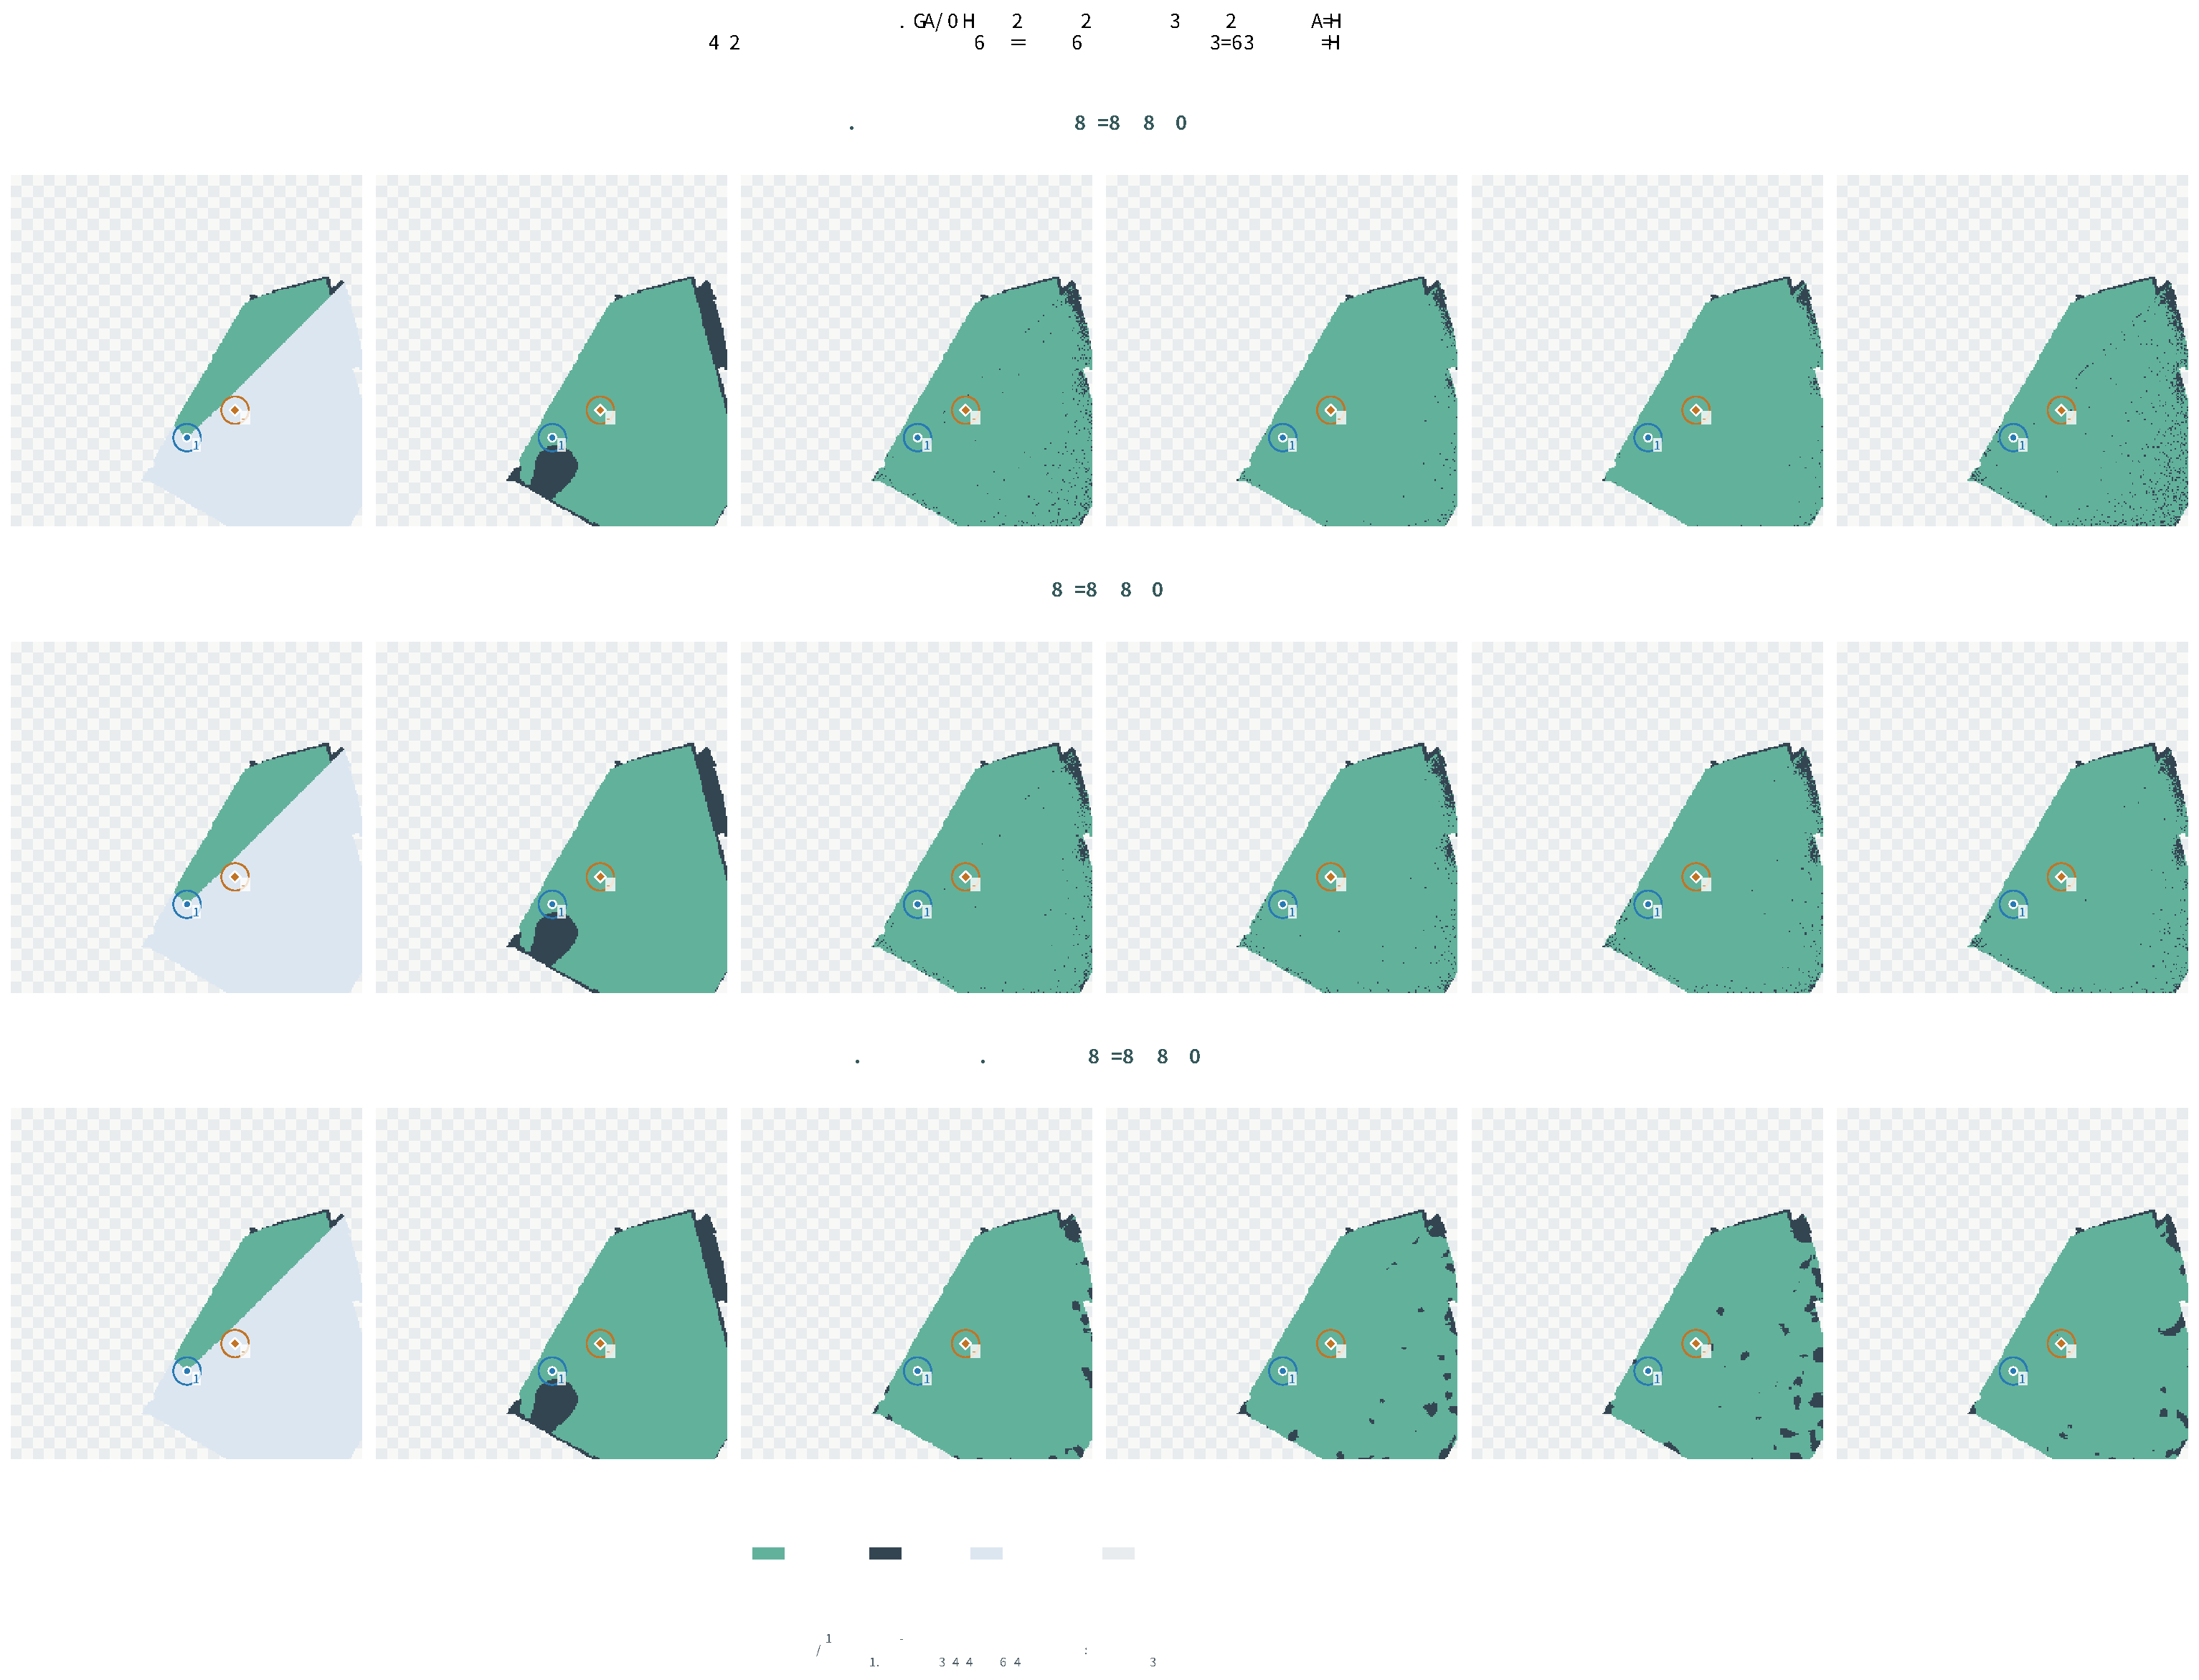
\includegraphics[width=.98\textwidth]{02_fixed_case_05.pdf}
\caption{Fixed archived gallery case 6: \texttt{obs\_101106:q011}, radius 10 grid cells, seed 20260910, validation-only. Same input and query across rows; first four stored worlds, with event frequencies from all 32. Original ConPath and independent are main development methods; the correlated categorical-noise variant is supplementary only. No outcome-based replacement or sample selection is performed.}
\end{figure}
\clearpage
\begin{figure}[H]\centering
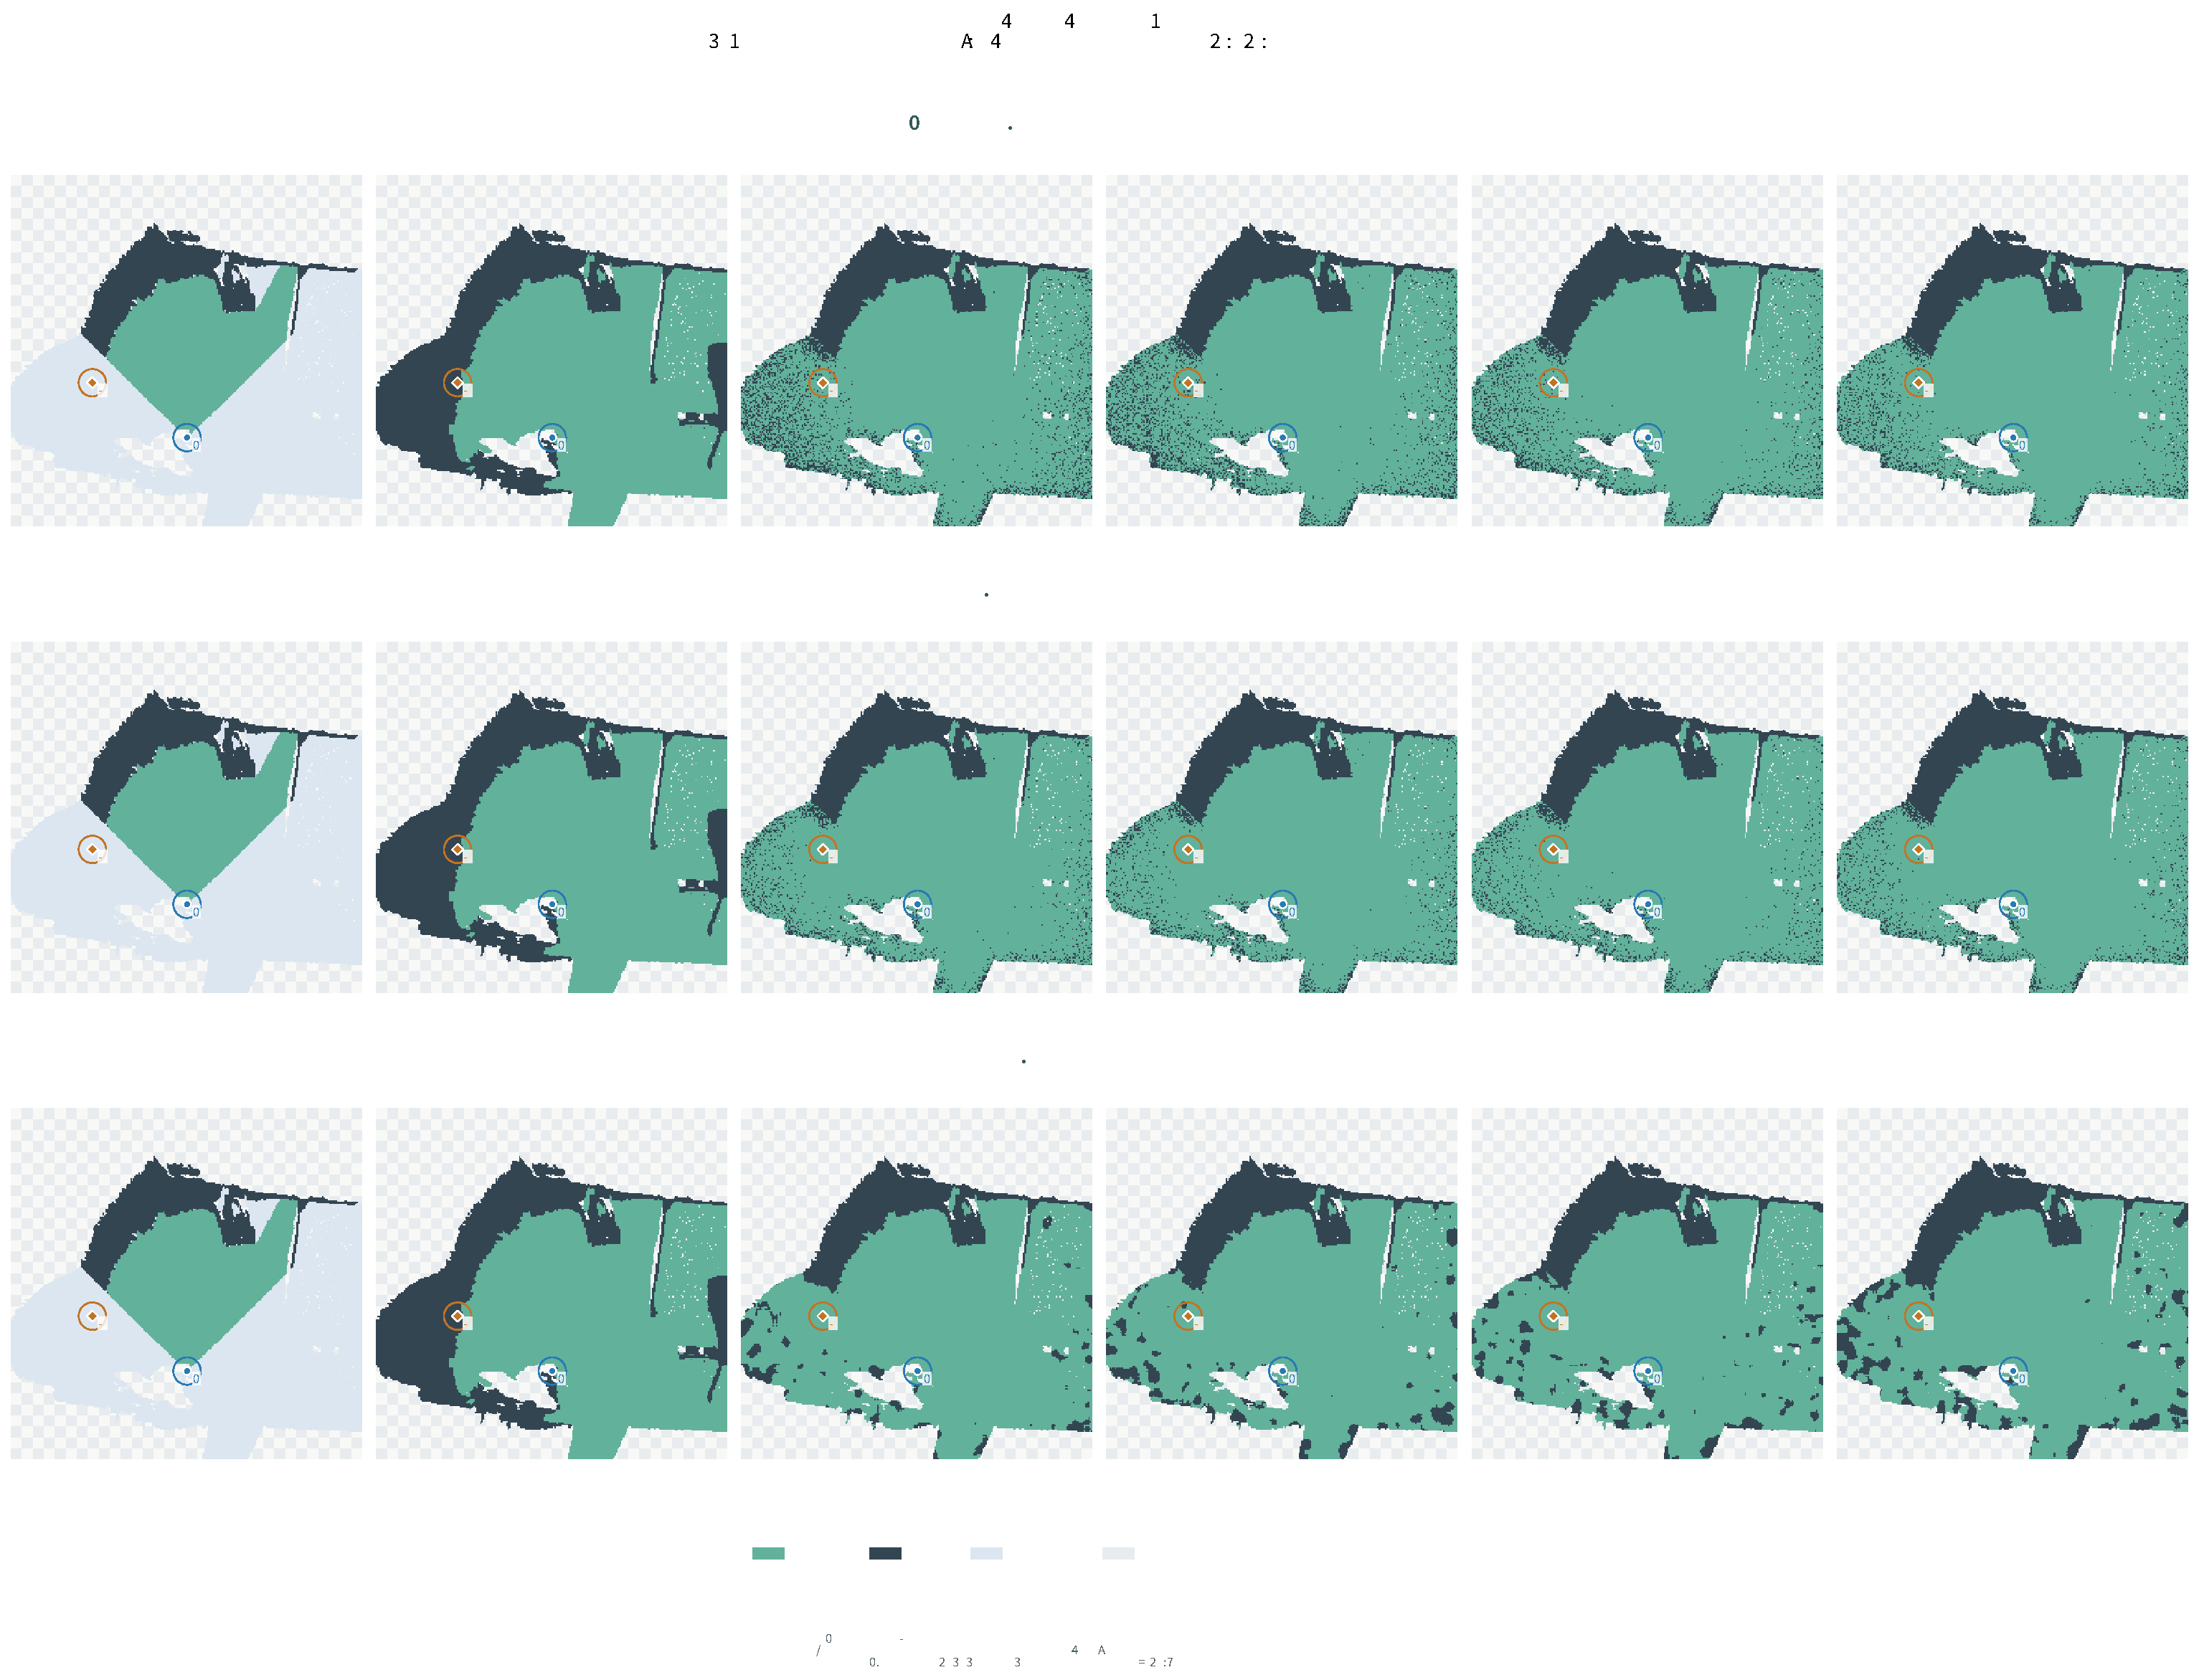
\includegraphics[width=.98\textwidth]{02_fixed_case_06.pdf}
\caption{Fixed archived gallery case 7: \texttt{obs\_166408:q019}, radius 10 grid cells, seed 20260910, validation-only. Same input and query across rows; first four stored worlds, with event frequencies from all 32. Original ConPath and independent are main development methods; the correlated categorical-noise variant is supplementary only. No outcome-based replacement or sample selection is performed.}
\end{figure}
\clearpage
\begin{figure}[H]\centering
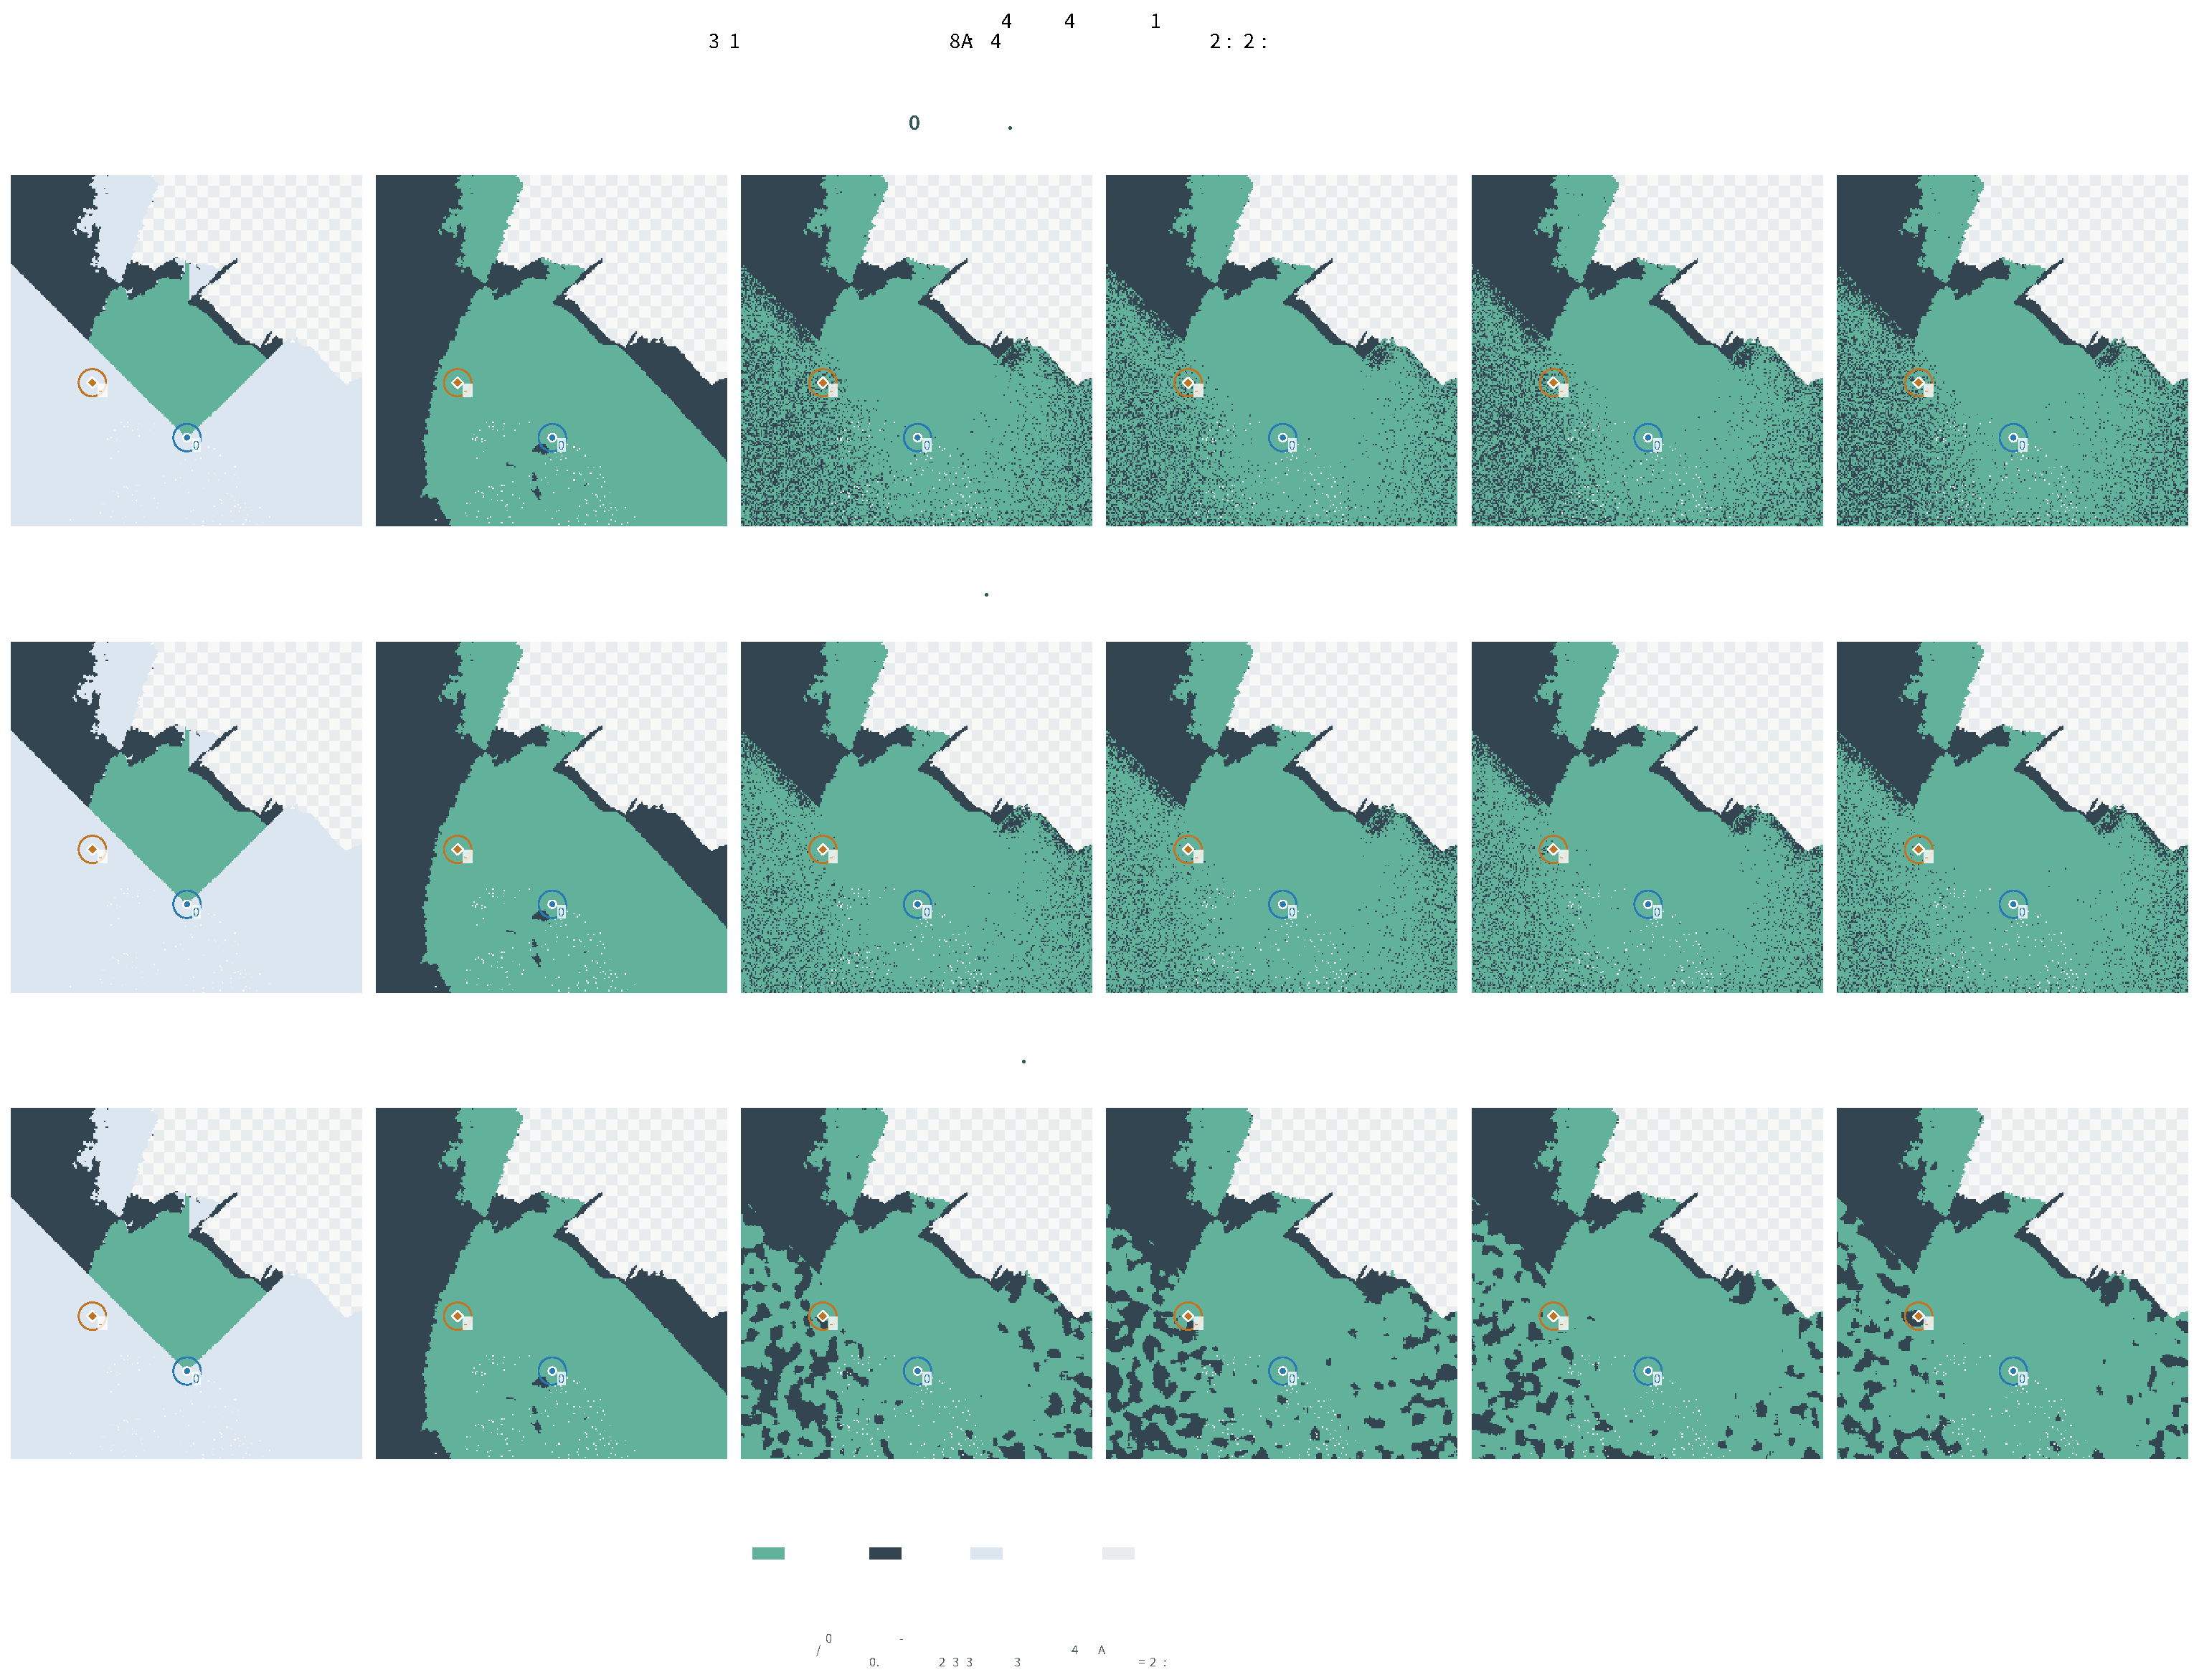
\includegraphics[width=.98\textwidth]{02_fixed_case_07.pdf}
\caption{Fixed archived gallery case 8: \texttt{obs\_157856:q019}, radius 10 grid cells, seed 20260910, validation-only. Same input and query across rows; first four stored worlds, with event frequencies from all 32. Original ConPath and independent are main development methods; the correlated categorical-noise variant is supplementary only. No outcome-based replacement or sample selection is performed.}
\end{figure}
\clearpage
\begin{figure}[H]\centering
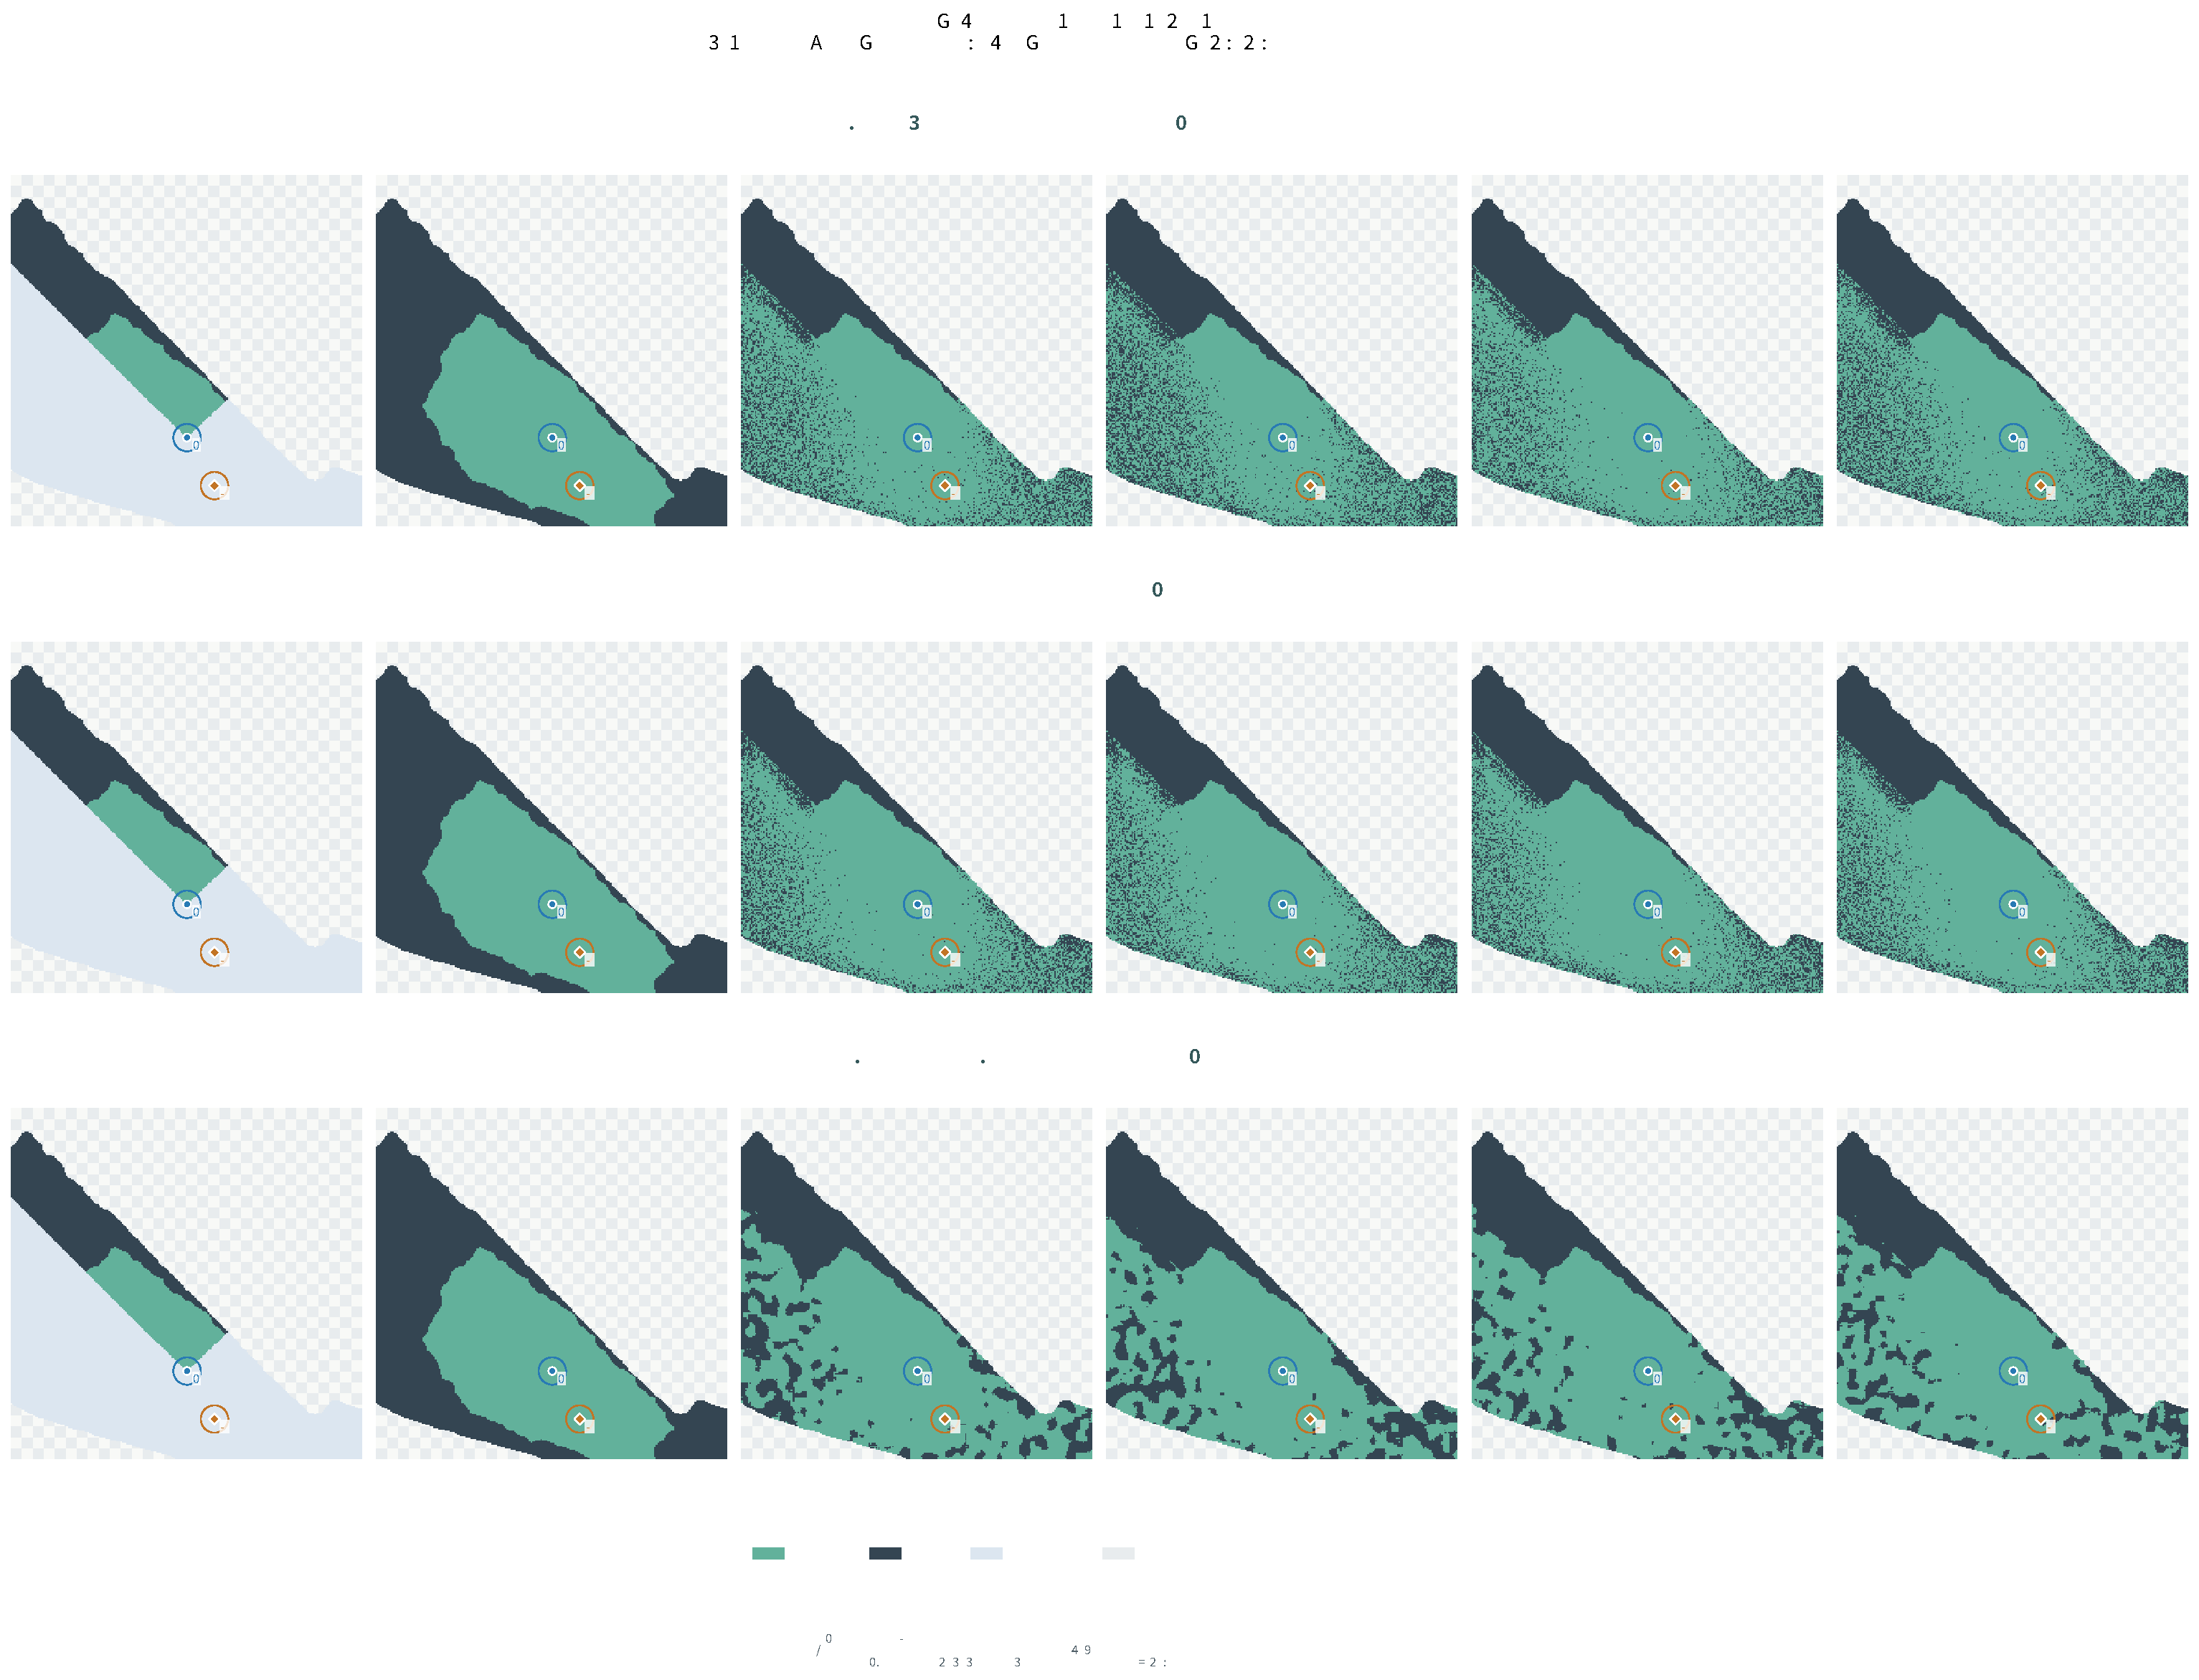
\includegraphics[width=.98\textwidth]{02_fixed_case_08.pdf}
\caption{Fixed archived gallery case 9: \texttt{obs\_203894:q002}, radius 10 grid cells, seed 20260910, validation-only. Same input and query across rows; first four stored worlds, with event frequencies from all 32. Original ConPath and independent are main development methods; the correlated categorical-noise variant is supplementary only. No outcome-based replacement or sample selection is performed.}
\end{figure}
\clearpage
\begin{figure}[H]\centering
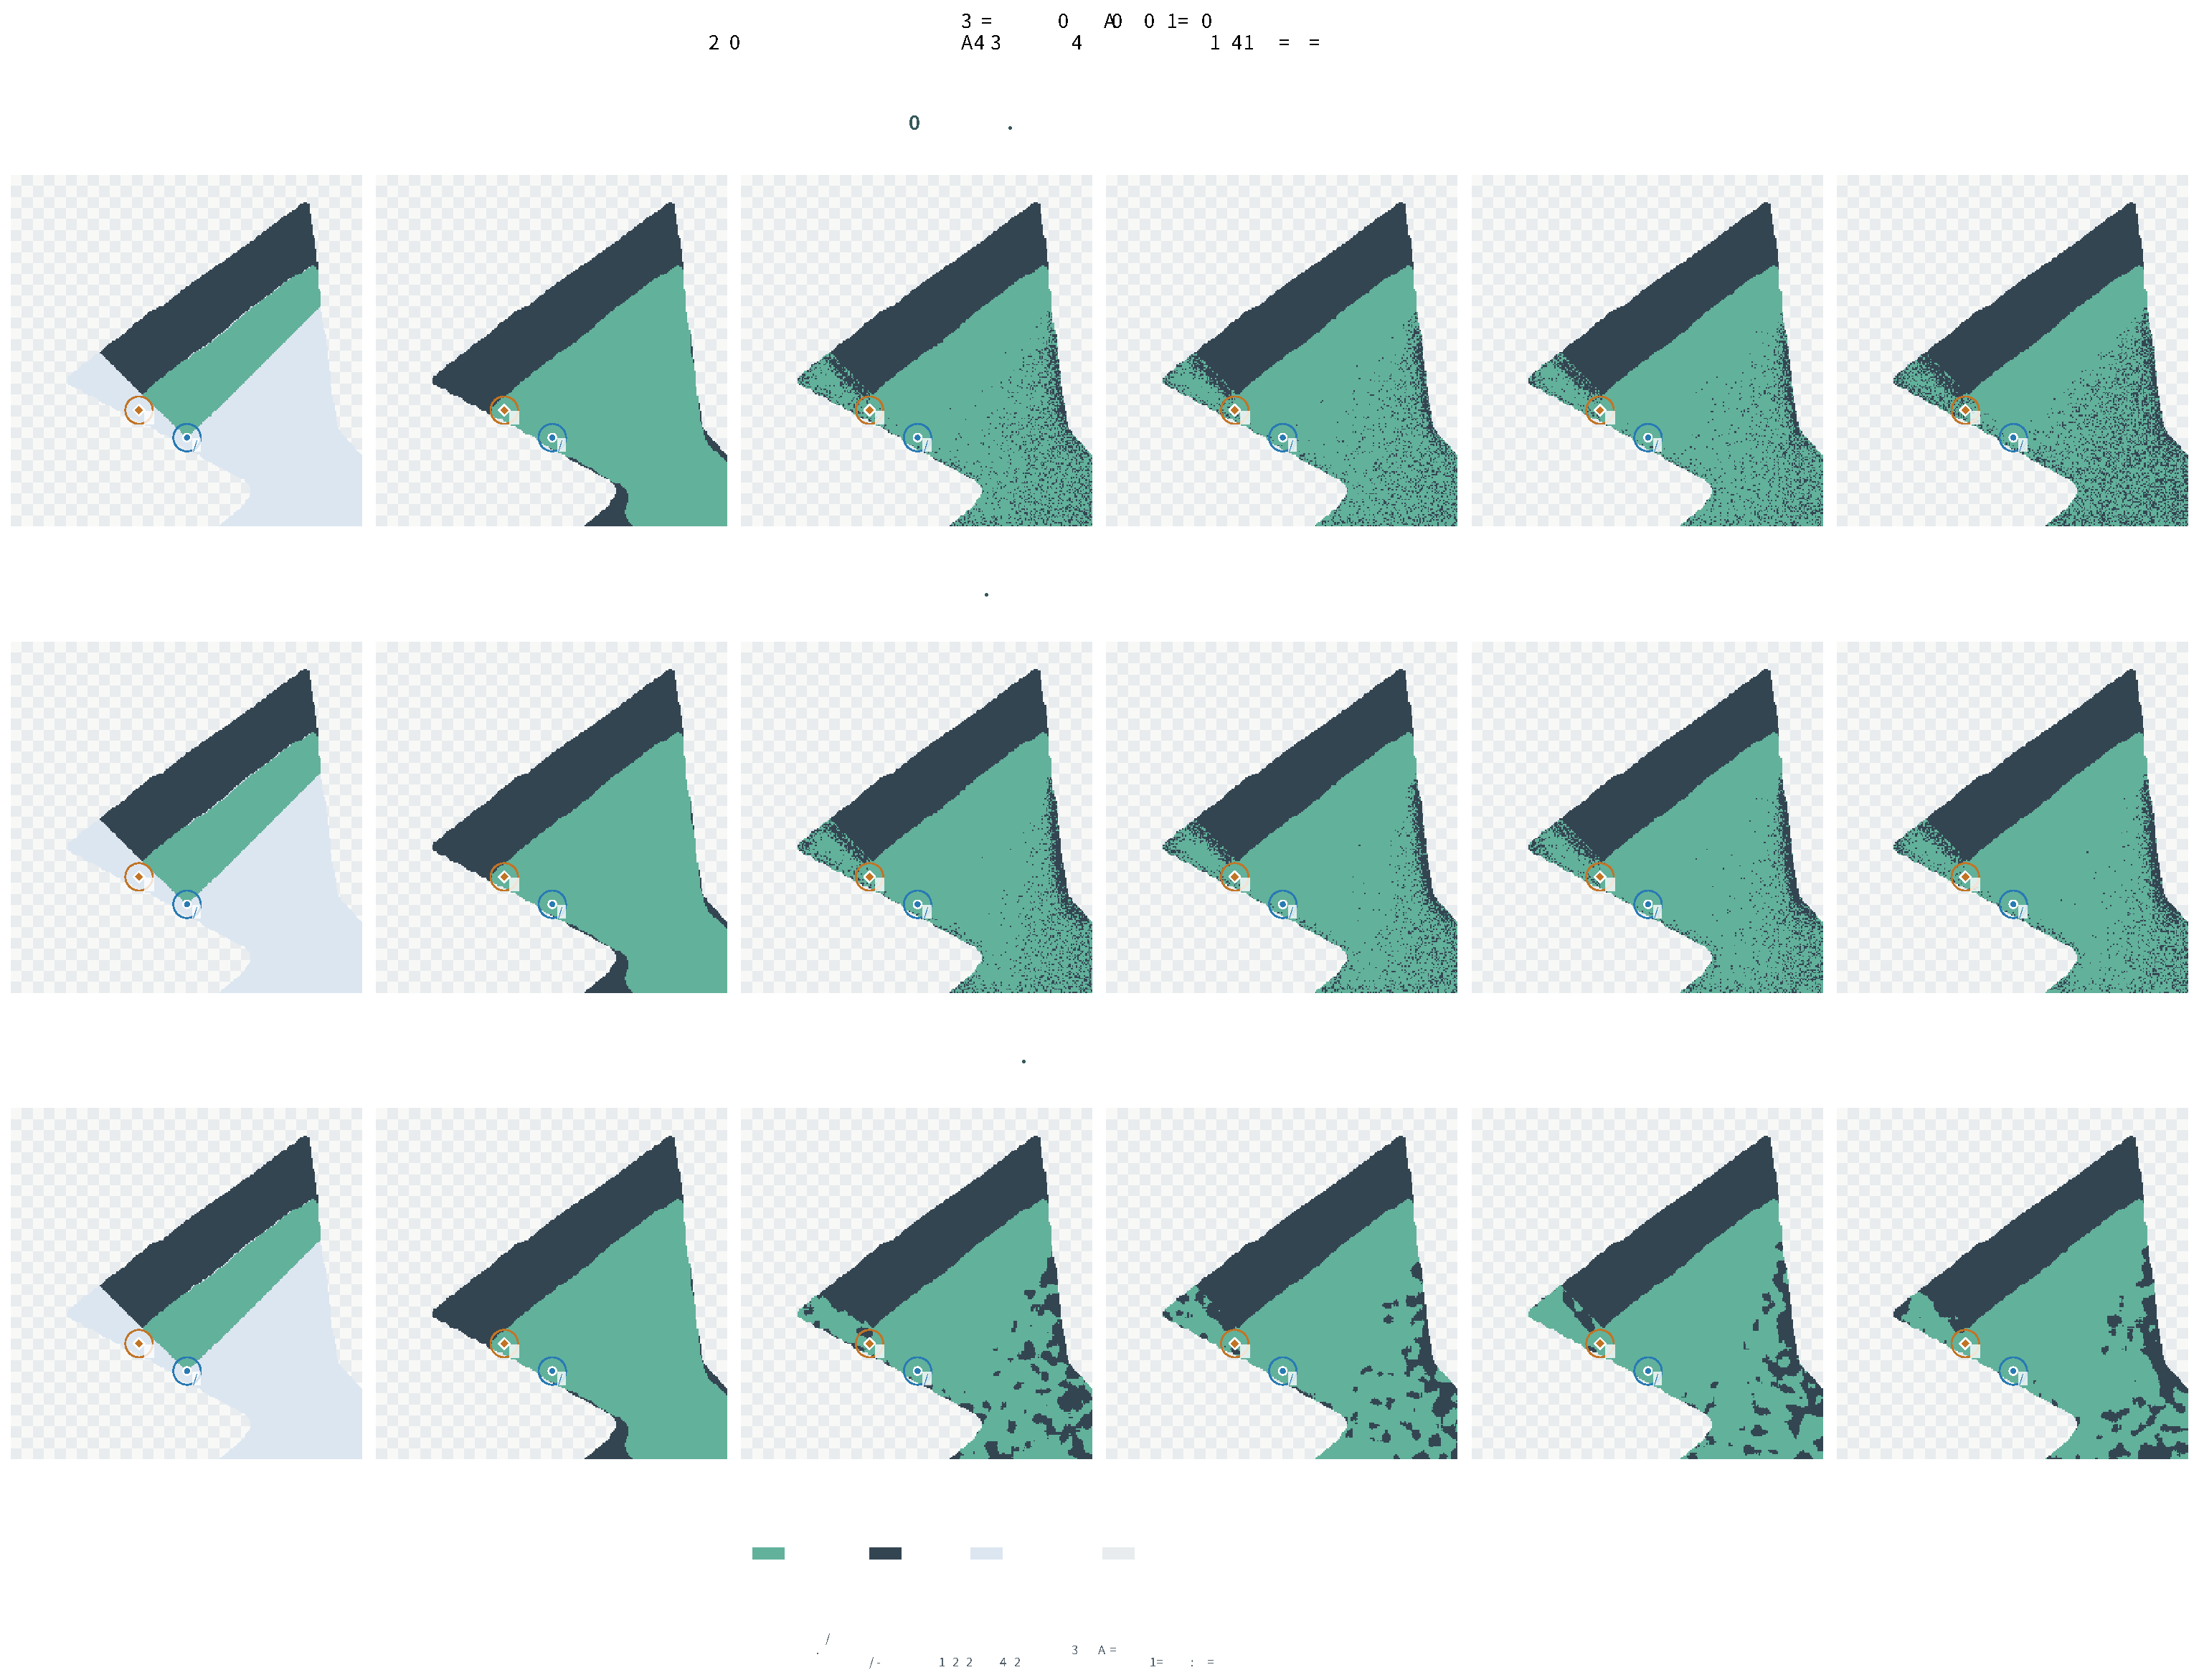
\includegraphics[width=.98\textwidth]{02_fixed_case_09.pdf}
\caption{Fixed archived gallery case 10: \texttt{obs\_173909:q007}, radius 10 grid cells, seed 20260910, validation-only. Same input and query across rows; first four stored worlds, with event frequencies from all 32. Original ConPath and independent are main development methods; the correlated categorical-noise variant is supplementary only. No outcome-based replacement or sample selection is performed.}
\end{figure}


\clearpage
\section{Test Access, Reproducibility, and Remaining Gaps}
No final test or \texttt{location\_6} has been opened for this consolidation or typesetting. Earlier FlatLands physical archive-test access included eight observations in historical training, five in historical validation, and 53 in an earlier query audit. These histories overlap and must not be summed as disjoint counts. An untouched physical-test claim is withdrawn. Final holdout eligibility requires a full access-history audit and exclusion of inspected parents; Boolean legacy flags do not establish it.

The current metadata-only inventory identifies a partial union of 1,532 development-exposed parent places across three recorded histories. External data preparation accessed 2,292 observations from 1,292 parents; its later quarantine excluded 34 observations from 19 parents, which remain previously inspected. This incomplete inventory does not certify other data as untouched. The old eight training and five validation physical-test observations are subsets of the 53-observation audit. The existing history also records 32 inspected ScanNet++ scenes; these counts are not added. None of these counts should be added to the 1,532-parent union. This audit uses saved metadata and does not open a new test manifest or test asset.

The principal source documents and the JSON/CSV validation snapshots are:
\begin{quote}\small\ttfamily
PAPER\_DRAFT.md\\
PAPER\_EVIDENCE.md\\
PAPER\_TABLES.md\\
PAPER\_FIGURES.md\\
results/FINAL\_MODEL\_SELECTION.md\\
results/paper\_validation\_snapshot.json\\
results/paper\_validation\_snapshot.csv
\end{quote}
The JSON snapshot has SHA-256
\begin{quote}\footnotesize\ttfamily
\nolinkurl{8a3b81ef1f01dec72e57f92d7c02d39ed0e3697e12389143a755a836cc4bbc32}.
\end{quote}
It contains 29 evidence rows, 23 current per-run metric records, and 189 source references. The typesetting manifest records source-document hashes, rendered table rows, and copied figure hashes. Underlying prediction/checkpoint/evaluator provenance remains in the original snapshot; no new model execution is necessary to rebuild the manuscript.

The current six-method matrix still lacks direct-query/no-event/no-global runs on D1. Historical direct-query has one seed. Calibration per-query files and strict bottleneck examples are unavailable. External models are under-converged and cancelled. The principal empirical support remains indoor BEV development, without outdoor, end-to-end sensor, robot closed-loop, or trajectory-output validation. Bounded gradients, finite samples, unresolved physical-scale calibration, incomplete convergence evidence, and the known zero-query weighting limitation remain. These are scientific limits, not typesetting errors.

The main document uses an IEEEtran conference-style layout. This work does not assert compliance with any unverified edition's page limit, anonymity policy, or submission formatting requirements. Authors and affiliations were not supplied and are not invented. Original Chinese plot labels are retained for current author review; a publication-ready language pass remains a presentation task, without authorization to alter experimental data or restart training.

\bibliographystyle{IEEEtran}
\bibliography{references}
\end{document}
